\bookpart{集合}{Sets}
\label{part:mathematical-language-analysis-optimization}
\label{part:sets}

\BookPartGuide{%
讨论一个问题时，首先要说清有哪些对象，以及对象之间可以建立什么联系。本部分回答两个问题：怎样描述集合与对象之间的联系，怎样比较集合的大小。它不依赖专门的前置知识，为全书各卷提供共同的表达语言。

第~\ref{chap:sets-relations-maps}章建立这套语言。集合确定对象的范围；关系记录哪些对象彼此相关，其中等价关系用来分类，偏序用来比较；映射要求每个输入恰好对应一个输出；索引族用编号保留同一对象的多次出现，从而能进行有限累计、归纳与递归。

第~\ref{chap:counting}章转而问有限集合有多少个元素，用双射、分类、分步、容斥和递推计算结果的个数。使用这些方法时，要先确定结果是否区分次序、是否允许重复、各部分有没有名称，再检查各类结果有无重叠或遗漏。

无限集合无法逐个数完，却仍能比较两边的元素能否一一配对。第~\ref{chap:cardinality}章用双射和单射比较集合大小，说明无限集合可以与真子集等势，并以可数性和对角线构造区分有理数与实数的大小。

阅读时注意区分三组概念：对象本身与它的编号或代表元；有序组与集合；元素个数（基数）与次序、几何长度。下一部分“实数与一元函数”从实数的确界与完备性出发研究极限、微分与积分，要用到本部分的映射、数列与可数性。卷二《向量、矩阵与多元微积分》用笛卡尔积和索引族表示向量、矩阵与多重下标，卷三《图》用集合、关系与计数描述图的结构与组合问题；后续的度量、测度与概率各卷还将反复使用可数并与可数性规则。}

\chapter{集合、关系与映射}
\label{chap:sets-functions-and-proofs}
\label{chap:sets-relations-maps}

设想一所学校开设四门课程，几名学生各自选了其中几门。拿到这份选课记录，会问：
哪些课程有人选，哪些课程两人都选了；某名学生与某门课程之间有没有选课联系；
怎样把每名学生对应到自己的选课；记录编号以后怎样汇总各门课的人数。
要据此推理和计算，需要先说清讨论哪些对象、对象之间有什么联系、
怎样把一个对象对应到另一个对象，以及怎样给一批对象编号并累计。

这四个问题依次对应集合、关系、映射与索引族，并且后一种工具由前一种搭建。
集合只回答“有哪些对象”，不记录次序；为了记录“谁与谁有联系”，需要有序对和笛卡尔积，关系就是笛卡尔积的子集。
映射是一种特殊的关系，它要求每个输入恰有一个输出；索引族又是以编号为输入的映射，它保留同一对象的多次出现，使有限累计成为可能。

本章只使用整数与实数的日常运算，不依赖专门的前置知识。
下一章用双射和有限累计计数，第~\ref{chap:cardinality}章再用单射与双射比较无限集合的大小；
实数本身的性质从第~\ref{chap:real-complex-functions}章开始建立。

\section{集合的定义与运算}
\label{sec:prelim-sets-relations-functions}

本节先说明怎样写出集合、怎样判断两个集合相等，再定义集合运算，
最后用已有集合构造幂集与笛卡尔积。

\subsection{集合的定义和描述}
\label{sec:prelim-set-definition}

\paragraph{集合与元素}
由一些确定的对象组成的整体称为\term{集合}（set），其中的对象称为它的元素；
“确定”是说任给一个对象，都能判断它是不是其中的元素。例如四门课程的编号组成集合$\{1,2,3,4\}$。
若$x$是集合$X$的元素，就说$x$属于$X$，记作$x\in X$；否则记作$x\notin X$。

集合只由它含有哪些元素决定：含有相同元素的两个集合相等，记作$X=Y$。
因此$\{1,2,3\}$、$\{3,2,1\}$与$\{1,1,2,3\}$是同一个集合。

不含任何元素的集合称为空集，记作$\varnothing$；只含一个元素$a$的集合$\{a\}$称为单元素集。

\paragraph{集合的描述}
列举法把元素逐个写在花括号中，例如$U=\{1,2,3,4\}$；
描述法写出挑选范围和所满足的条件，例如$U=\{i\in\mathbb Z:1\leq i\leq4\}$，
冒号读作“使得”，冒号前的$i\in\mathbb Z$表示从整数中挑选。

挑选范围不能省略：同一条件下从实数中挑选，得到的是区间$\{x\in\mathbb R:1\leq x\leq4\}=[1,4]$。

本书用$\mathbb N=\{0,1,2,\ldots\}$表示自然数集合，$\mathbb N_+=\{1,2,\ldots\}$表示正整数集合，
$\mathbb Z$、$\mathbb Q$和$\mathbb R$分别表示整数、有理数与实数集合。
区间$[a,b]$包含两个端点，$(a,b)$不含端点，$[a,b)$与$(a,b]$各只含一个端点。

\paragraph{子集}
若$A$的每个元素都属于$B$，就称$A$是$B$的子集（subset），记作$A\subseteq B$；
若还有$A\neq B$，就称$A$是$B$的真子集，记作$A\subsetneq B$。

属于与包含比较的对象不同：$1\in U$说的是编号$1$属于$U$，$\{1\}\subseteq U$说的是集合$\{1\}$包含于$U$；
$\{1,2\}\subseteq U$成立，$\{1,2\}\in U$却不成立，因为$U$的元素是编号而不是集合。

空集是任何集合的子集，因为“它的每个元素都属于$B$”无从违反。

由于集合只由元素决定，$A=B$当且仅当$A\subseteq B$且$B\subseteq A$；
证明集合相等时，常把等式拆成这两个包含分别验证，称为双向包含。

\subsection{集合的运算}
\label{sec:prelim-set-operations}

\paragraph{基本运算}
设甲、乙两名学生的选课分别是$C=\{1,2,3\}$与$D=\{2,3,4\}$，以全部课程$U=\{1,2,3,4\}$为全集。
合并名单、找共同课程、排除已知课程，分别对应下面的运算。
\begin{itemize}
 \item 并集：$X\cup Y=\{x:x\in X\text{ 或 }x\in Y\}$，“或”允许两个条件同时成立。例如$C\cup D=\{1,2,3,4\}$。
 \item 交集：$X\cap Y=\{x:x\in X\text{ 且 }x\in Y\}$，例如$C\cap D=\{2,3\}$。若$X\cap Y=\varnothing$，称$X$与$Y$不交。
 \item 差集：$X\setminus Y=\{x:x\in X\text{ 且 }x\notin Y\}$，例如$C\setminus D=\{1\}$，而$D\setminus C=\{4\}$。
 \item 对称差：$X\mathbin{\triangle}Y=(X\setminus Y)\cup(Y\setminus X)$，即恰好属于其中一个集合的元素，例如$C\mathbin{\triangle}D=\{1,4\}$。
 \item 补集：对全集$U$的子集$X$，$X^{\mathrm c}=U\setminus X$，例如$C^{\mathrm c}=\{4\}$。
       补集依赖全集：若全集换成$\{1,2,3,4,5\}$，$C$的补集就变成$\{4,5\}$。
\end{itemize}

\paragraph{运算律}
这些运算都由成员条件定义，运算律可以逐个元素核对。交与并满足交换律、结合律与分配律：
\begin{align*}
 X\cap Y&=Y\cap X,\\
 X\cup Y&=Y\cup X,\\
 (X\cap Y)\cap Z&=X\cap(Y\cap Z),\\
 (X\cup Y)\cup Z&=X\cup(Y\cup Z),\\
 X\cap(Y\cup Z)&=(X\cap Y)\cup(X\cap Z),\\
 X\cup(Y\cap Z)&=(X\cup Y)\cap(X\cup Z).
\end{align*}

前四式来自“且”“或”可以交换次序、改变组合方式。以第五式为例，左边要求$x\in X$，并且$x$属于$Y$或$Z$；
这恰好是说$x$同时属于$X$与$Y$，或者同时属于$X$与$Z$。

补集与交、并的关系由下面的定理给出。
\begin{theorem}[De Morgan律]
\label{thm:sets-de-morgan}
设$X,Y$是全集$U$的子集，则
\begin{equation}
 (X\cup Y)^{\mathrm c}=X^{\mathrm c}\cap Y^{\mathrm c},\qquad
 (X\cap Y)^{\mathrm c}=X^{\mathrm c}\cup Y^{\mathrm c}.
 \label{eq:prelim-de-morgan-two-sets}
\end{equation}
\end{theorem}
\begin{proof}
用双向包含证明第一式。若$u\in(X\cup Y)^{\mathrm c}$，则$u\notin X\cup Y$，因而$u\notin X$且$u\notin Y$，
即$u\in X^{\mathrm c}\cap Y^{\mathrm c}$。

反过来，若$u\in X^{\mathrm c}\cap Y^{\mathrm c}$，则$u$既不属于$X$也不属于$Y$，
因而$u\notin X\cup Y$，即$u\in(X\cup Y)^{\mathrm c}$。

第二式同理：$u\notin X\cap Y$当且仅当$u\notin X$或$u\notin Y$，即$u\in X^{\mathrm c}\cup Y^{\mathrm c}$。
\end{proof}
第一式说的是，“不满足任何一个条件”与“每个条件都不满足”是同一件事；下一章计数违反限制的结果时要用到它。

\paragraph{差集的次序}
差集既没有交换律，也没有结合律。
\begin{example}[差集不满足交换律与结合律]
\label{ex:sets-difference-order}
前面已有$C\setminus D\neq D\setminus C$。再取$E=\{1\}$，先求$C\setminus D$与先求$D\setminus E$得到不同的结果：
\[
 \begin{aligned}
  (C\setminus D)\setminus E&=\{1\}\setminus\{1\}=\varnothing,\\
  C\setminus(D\setminus E)&=C\setminus D=\{1\}.
 \end{aligned}
\]
第二行用到$D\setminus E=D$，因为$1\notin D$。
\end{example}
所以连续求差时必须用括号标明先后。

\subsection{幂集、笛卡尔积与有序组}
\label{sec:sets-power-sets-products}

前面的运算得到的仍是原全集的子集。把一名学生的全部选课当成一个对象，
或者把“先选一门、再选一门”记录成一个对象，则需要构造新的集合。

\paragraph{幂集}
集合$X$的全部子集组成的集合称为$X$的\term{幂集}（power set），记作
\[
 \mathcal P(X)=\{A:A\subseteq X\}.
\]
例如$\mathcal P(\{1,2\})=\{\varnothing,\{1\},\{2\},\{1,2\}\}$，一名学生的全部可能选课就是课程集合的幂集。

幂集的元素是集合：$\{1\}\in\mathcal P(\{1,2\})$，而$1$不是$\mathcal P(\{1,2\})$的元素。

以集合为元素的集合也称为\term{集合族}（set family），它不必收集全部子集，例如$\{\{1\},\{2\}\}\subseteq\mathcal P(\{1,2\})$。

\paragraph{有序对与笛卡尔积}
集合不记录次序，有序对$(x,y)$则保留两个位置：$(x,y)=(x',y')$要求$x=x'$且$y=y'$。
所以$(1,2)\neq(2,1)$，而$\{1,2\}=\{2,1\}$；有序对还允许两个位置相同，如$(1,1)$。
第一个位置取自$X$、第二个位置取自$Y$的全部有序对组成\term{笛卡尔积}（Cartesian product）
\begin{equation}
 X\times Y=\{(x,y):x\in X,\ y\in Y\}.
 \label{eq:sets-cartesian-product}
\end{equation}
例如，两个因子分别取$\{1,2\}$与$\{a,b\}$时，
\[
 \{1,2\}\times\{a,b\}=\{(1,a),(1,b),(2,a),(2,b)\}.
\]
当$X,Y$都非空且$X\neq Y$时，$X\times Y\neq Y\times X$。

回到选课：一名学生“先报一门首选课、再报一门备选课”，记录$(1,3)$与$(3,1)$表示不同的报名，
它们都属于$U\times U$；若只问他报了哪些课，两者给出同一个集合$\{1,3\}$。

$U\times U$中还有$(2,2)$这样的记录，它表示两次报了同一门课，而集合$\{2,2\}=\{2\}$已看不出报了两次。
下一章的计数正是从“记录有序组还是记录集合”这一区别出发的。

一般地，有序$d$元组$(x_1,\ldots,x_d)$的第$i$个位置称为第$i$个坐标，两个$d$元组相等当且仅当对应坐标逐一相等。
第$i$个坐标取自$X_i$的全部$d$元组组成$X_1\times\cdots\times X_d$，各因子相同时记为$X^d$；
特别地，$\mathbb R^d$是全部有序$d$元实数组的集合，$\mathbb R^2$就是平面上点的坐标。
映射$(x_1,\ldots,x_d)\mapsto x_i$称为第$i$个投影。

\section{关系与分类}
\label{sec:prelim-binary-relations}

“学生选了某门课”“$1$不大于$2$”“两个整数除以$3$的余数相同”，问的都是一对对象是否满足某个条件。
本节把这样的条件写成有序对的集合，研究关系的性质，再用两类特殊的关系分类和比较。

\subsection{二元关系及其性质}
\label{sec:prelim-binary-relation-definition}
\label{sec:prelim-relation-properties}

\paragraph{二元关系}
设三名学生$s_1,s_2,s_3$中，$s_1$选了课程$1,2,3$，$s_2$选了$2,3,4$，$s_3$没有选课。
选课情况是笛卡尔积$\{s_1,s_2,s_3\}\times\{1,2,3,4\}$的子集
\[
 R=\{(s_1,1),(s_1,2),(s_1,3),(s_2,2),(s_2,3),(s_2,4)\}.
\]
一般地，笛卡尔积的任一子集$R\subseteq X\times Y$称为$X$到$Y$的\term{二元关系}（binary relation），
写$xRy$表示$(x,y)\in R$；$X=Y$时称$R$为$X$上的关系。

至少与一个$y$有关系的$x$组成$R$的定义域，至少与一个$x$有关系的$y$组成$R$的值域；
上例的定义域是$\{s_1,s_2\}$，值域是全部四门课程。

同一对集合之间可以有许多关系，空集和整个积也是关系。
关系也不要求每个$x$恰好对应一个$y$：$s_1$对应三门课，$s_3$一门也不对应。后面的映射正是对这一点加以限制。

$X$上的关系可以画成箭头图：把$X$的元素画成点，$xRy$时从$x$画一支箭头指向$y$，$xRx$画成从$x$回到自身的环。
下面的各种性质都可以在箭头图上读出，例如对称性就是每支箭头都有反向箭头。

\paragraph{关系的基本性质}
设$R$是集合$X$上的关系。
若每个$x\in X$都有$xRx$，称$R$具有\term{自反性}（reflexivity）；
若$xRy$总蕴含$yRx$，称$R$具有\term{对称性}（symmetry）；
若$xRy$与$yRx$只在$x=y$时同时成立，称$R$具有\term{反对称性}（antisymmetry）；
若$xRy$且$yRz$总蕴含$xRz$，称$R$具有\term{传递性}（transitivity）。

用三个熟悉的关系核对。相等关系具有上述四种性质，因为它只关联同一个对象。

实数上的$\leq$具有自反性、反对称性和传递性，但不具有对称性：$1\leq2$，而$2\not\leq1$。

\begin{example}[整除关系的性质]
\label{ex:sets-divisibility-properties}
正整数上的整除关系$a\mid b$表示存在正整数$c$使$b=ac$。它具有自反性，因为$a=a\cdot1$；
也具有传递性，因为$b=ac$、$e=bc'$推出$e=a(cc')$；还具有反对称性，因为$a\mid b$且$b\mid a$时$a\leq b\leq a$。

它不具有对称性：例如$2\mid4$，但$4\nmid2$。若把整除关系放到非零整数上，$2\mid-2$且$-2\mid2$，反对称性就不再成立。
\end{example}
最后一例说明，同一条规则是否具有某种性质，还取决于在哪个集合上讨论。

反对称性不是对称性的否定。若$xRy$成立时$yRx$总不成立，称$R$具有\term{非对称性}（asymmetry），
例如实数上的$<$；$\leq$不是非对称的，因为$1\leq1$。非对称关系一定反对称，
并且没有$x$满足$xRx$，即具有\term{反自反性}（irreflexivity）；反对称关系则允许$xRx$。

\paragraph{关系的闭包}
一个关系缺少某种性质时，可以补入必要的有序对。包含$R$、具有指定性质、并且在包含意义下最小的关系，
称为相应的\term{关系闭包}（closure of a relation）；“最小”是说任何包含$R$并具有该性质的关系都包含它。
反对称性不能靠补入有序对获得，因为已有的双向关联无法去掉。

自反闭包是$R\cup\{(x,x):x\in X\}$，对称闭包是$R\cup\{(y,x):(x,y)\in R\}$，补入的都是满足性质所必需的有序对。
例如$\{1,2,3\}$上的$\{(1,2),(2,3)\}$，自反闭包补入$(1,1),(2,2),(3,3)$，对称闭包补入$(2,1),(3,2)$。

传递闭包$R^+$规定：$xR^+y$当且仅当存在有限链$x=x_0,x_1,\ldots,x_n=y$（$n\geq1$），每一步都有$x_{k-1}Rx_k$。
两条链首尾相接仍是链，所以$R^+$传递；任何包含$R$的传递关系沿链使用传递性，都含有链的首尾对，所以$R^+$最小。
上例的传递闭包只需补入$(1,3)$。

\subsection{等价关系、划分与商集}
\label{sec:prelim-equivalence-relations}

\paragraph{等价关系}
按除以$3$的余数可以把整数分成三组。“分在同一组”这一关系应当满足：每个整数与自己同组；
$x$与$y$同组时$y$与$x$也同组；$x$与$y$、$y$与$z$分别同组时$x$与$z$也同组。这正是自反、对称与传递性。
\begin{definition}[等价关系]
\label{def:prelim-equivalence-relation}
设$R$是集合$X$上的关系。若$R$具有自反性、对称性与传递性，就称$R$为\term{等价关系}（equivalence relation）。
对$x\in X$，与$x$等价的元素组成$x$的\term{等价类}（equivalence class）
$[x]_R=\{y\in X:yRx\}$，$x$称为这个等价类的一个代表元。
\end{definition}
\begin{example}[按除以$3$的余数分类]
\label{ex:sets-congruence-mod-three}
整数上的关系“$3$整除$x-y$”是等价关系：$x-x=0$；$x-y$是$3$的倍数时$y-x$也是；
$x-y$与$y-z$都是$3$的倍数时，它们的和$x-z$也是。它有三个等价类$[0],[1],[2]$，而$[3]=[0]$，
同一个等价类可以由不同的代表元写出。
\end{example}

\paragraph{等价类与划分}
若$X$的一族非空子集两两不交，并且它们的并等于$X$，就称这族子集为$X$的一个\term{划分}（partition）。
等价关系恰好给出划分。
\begin{theorem}[等价类构成划分]
\label{thm:sets-equivalence-partition}
设$R$是集合$X$上的等价关系，则全部等价类组成$X$的一个划分；并且对$x,y\in X$，或者$[x]_R=[y]_R$，或者$[x]_R\cap[y]_R=\varnothing$。
反过来，$X$的每个划分都由唯一的等价关系这样给出，即“属于同一块”。
\end{theorem}
\begin{proof}
由自反性，$x\in[x]_R$，所以每个等价类非空，并且各等价类的并是$X$。

再证明有公共元素的两个等价类相等。设$z\in[x]_R\cap[y]_R$，即$zRx$且$zRy$。由对称性得$xRz$，再由传递性得$xRy$。
于是任取$u\in[x]_R$，由$uRx$与$xRy$得$uRy$，即$u\in[y]_R$，所以$[x]_R\subseteq[y]_R$；交换$x,y$得反向包含。
因此不同的等价类两两不交，全部等价类构成划分。

反过来，给定划分，令$xRy$当且仅当$x,y$属于同一块，三条性质直接成立，其等价类就是各块；
而任何以这些块为等价类的等价关系都必须如此定义，所以它唯一。
\end{proof}
因此，在同一个集合上给出等价关系与给出划分是同一件事的两种写法。

\paragraph{商集}
分组以后，常把每一组当作一个新对象。全部等价类组成的集合记为$X/R$，称为商集（quotient set）。
对整数按除以$3$的余数分组，商集是$\{[0],[1],[2]\}$；它的三个元素都是整数的子集，不是整数，
$0,1,2$只是用来写出它们的代表元。

正因为代表元只是记法，在商集上定义运算或映射时，必须检查结果不依赖代表元的选取。
\begin{example}[商集上的规定是否依赖代表元]
\label{ex:sets-quotient-well-defined}
规定$[a]+[b]=[a+b]$：若$a'\in[a]$、$b'\in[b]$，则$(a'+b')-(a+b)$仍是$3$的倍数，结果不变，所以这一加法有意义。

规定“$[a]$的奇偶性就是$a$的奇偶性”则不行：$0$与$3$代表同一个等价类，奇偶性却不同。
\end{example}

商集的元素也可以有几何含义。
\begin{example}[平面非零点按比例分类]
\label{ex:sets-proportional-points}
在平面上除原点以外的点中，规定$P\sim Q$当且仅当存在非零实数$c$使$P=cQ$，
这是等价关系，每个等价类是一条过原点的直线去掉原点；若只允许$c>0$，同一直线在原点两侧的部分分属两个类。
\end{example}
图~\ref{fig:vol1-add-equivalence-directions}比较这两种分类。
\begin{figure}[!htb]
  \centering
  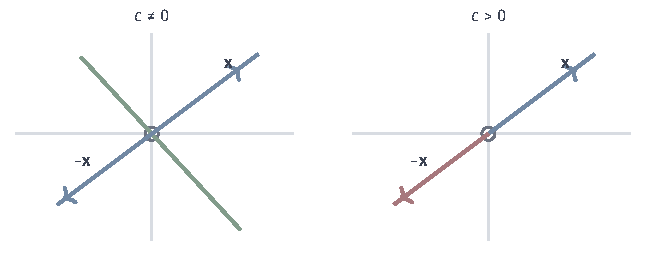
\includegraphics[width=112mm]{figures/00-shared/mathematical-preliminaries-upper/00-shared/tikz/mathematical-language-combinatorics-analysis-optimization-comprehension-additions/equivalence-directions.pdf}
  \caption{平面中非原点的等价分类。每支箭头从原点指向一个点。左侧允许非零实比例，同一直线上的点属于同一类；右侧只允许正比例，同一直线的两侧分成蓝、红两类。绿色表示另一条直线上的类；空心原点不属于被分类的集合。}
  \label{fig:vol1-add-equivalence-directions}
\end{figure}

\subsection{偏序、全序与极值元素}
\label{sec:prelim-order-relations}

\paragraph{偏序与全序}
子集之间可以按包含比较，正整数之间可以按整除比较，但$\{1\}$与$\{2\}$互不包含，$2$与$3$互不整除。
这类比较关系都具有自反性、反对称性与传递性。
\begin{definition}[偏序关系]
\label{def:prelim-partial-order}
集合$X$上具有自反性、反对称性与传递性的关系称为\term{偏序关系}（partial order），常记作$\preceq$，
配备了偏序的集合记作$(X,\preceq)$。若$x\preceq y$与$y\preceq x$至少有一个成立，称$x$与$y$可比较。
若$X$中任意两个元素都可比较，则称$\preceq$为\term{全序}（total order）。
\end{definition}
实数上的$\leq$是全序，包含关系与整除关系只是偏序。

\paragraph{最小元与极小元}
设$A\subseteq X$非空。若$a\in A$满足$a\preceq b$对每个$b\in A$成立，称$a$为$A$的\term{最小元}（least element）；
若$b\preceq a$对每个$b\in A$成立，称$a$为\term{最大元}（greatest element）。
若$b\in A$且$b\preceq a$必有$b=a$，即$A$中没有比$a$更小的元素，称$a$为\term{极小元}（minimal element）；
若$b\in A$且$a\preceq b$必有$b=a$，称$a$为\term{极大元}（maximal element）。

\begin{example}[有极小元而无最小元]
\label{ex:sets-minimal-not-least}
在整除偏序下取$A=\{2,3,4,6\}$：$2,3$都是极小元，$4,6$都是极大元，但$A$没有最小元和最大元，因为$2$与$3$不可比，$4$与$6$也不可比。
\end{example}
最小元若存在则唯一：两个最小元彼此不大于对方，由反对称性相等。最小元一定是极小元；在全序中，极小元也是最小元。

\paragraph{上界与下界}
若$u\in X$满足$a\preceq u$对每个$a\in A$成立，称$u$为$A$的\term{上界}（upper bound）；
若$l\in X$满足$l\preceq a$对每个$a\in A$成立，称$l$为$A$的\term{下界}（lower bound）。

与最值元素不同，界不必属于$A$：例~\ref{ex:sets-minimal-not-least}中$12$是$A$的上界，$1$是下界，都不在$A$中。
上界与下界也往往不唯一：$24$、$36$同样是这个$A$的上界。

\paragraph{上确界与下确界}
上界有许多个时，自然要问其中有没有最紧的一个。若$A$的上界组成的集合有最小元$\beta$，
就称$\beta$为$A$的\term{上确界}（supremum），记作$\sup A$；类似地，下界组成的集合若有最大元，称它为$A$的\term{下确界}（infimum），记作$\inf A$。
由最小元的唯一性，确界若存在则唯一。

在整除偏序下，例~\ref{ex:sets-minimal-not-least}中$A=\{2,3,4,6\}$的上界是$2,3,4,6$的公倍数，也就是$12$的全部倍数，
它们在整除意义下以$12$为最小，所以$\sup A=12$；下界是$2,3,4,6$的公因数，只有$1$，所以$\inf A=1$。
这两个确界都不属于$A$，而$A$也没有最大元与最小元。

若$\sup A$属于$A$，它就是$A$的最大元；反过来，最大元若存在，它也是上确界，因为它是上界，并且任何上界都不小于它。
所以确界是比最值更弱的要求：最值要求集合内部有最紧的元素，确界只要求集合外部的界中有最紧的一个。

一般偏序并不保证确界存在。例如在有理数集合$(\mathbb Q,\leq)$中，满足$x^2<2$的有理数组成的集合有上界，却没有有理数上确界；
这一断言及实数中确界存在的原理在第~\ref{sec:ru-supremum-completeness}节建立，并由此引出实数的完备性。

\section{映射}
\label{sec:prelim-functions-value-ranges}

关系允许一个对象对应多个对象，也允许不对应任何对象。“每名学生的学号”“每个实数的平方”则要求每个输入恰好得到一个输出。
本节定义映射，研究像与原像，按能否逐一配对给映射分类，最后讨论复合映射与逆映射。

\subsection{映射、像与原像}
\label{sec:prelim-function-definition}

\paragraph{映射的定义}
设$X,Y$是两个集合。若$X$到$Y$的关系使每个$x\in X$恰好与一个$y\in Y$有关系，
就称它为$X$到$Y$的\term{映射}（map），也称\term{函数}（function），记作$f:X\to Y$；
与$x$对应的元素记作$f(x)$，记号$x\mapsto f(x)$读作“把$x$对应到$f(x)$”。

$X$称为定义域或源集，$Y$称为陪域或目标集，集合$\{(x,f(x)):x\in X\}$称为$f$的图像（graph）。
实际取得的输出组成$f(X)=\{f(x):x\in X\}$，称为值域或像集，它是目标集的子集。

给出映射要同时说明源集、目标集和对应规则。同一规则$x\mapsto x^2$可以给出$\mathbb R\to\mathbb R$与$\mathbb R\to[0,\infty)$两个映射，
值域都是$[0,\infty)$，但前者的目标集中还有取不到的负数。两个映射相等，要求源集、目标集分别相同，且在每个输入处取值相同。

从$X$到$Y$的全部映射组成的集合记为$Y^X$，例如$\{0,1\}^{\{1,2\}}$有四个元素，由$(f(1),f(2))$的四种取值确定。

\paragraph{像与原像}
对映射$f:X\to Y$，可以问一组输入得到哪些输出，也可以问一组输出来自哪些输入。
对$A\subseteq X$与$B\subseteq Y$，分别定义$A$的像与$B$的\term{原像}（preimage）：
\begin{align}
 f(A)&=\{f(x):x\in A\}\subseteq Y,\notag\\
 f^{-1}(B)&=\{x\in X:f(x)\in B\}\subseteq X.
 \label{eq:prelim-preimage}
\end{align}

以平方映射$f:\mathbb R\to\mathbb R$为例：
\begin{align*}
 f(\{-2,1\})&=\{1,4\},\\
 f^{-1}(\{1\})&=\{-1,1\},\\
 f^{-1}([1,4])&=[-2,-1]\cup[1,2],\\
 f^{-1}(\{-1\})&=\varnothing.
\end{align*}

原像是集合，可以含多个元素，也可以为空；记号$f^{-1}(B)$并不要求$f$有逆映射。
原像与集合运算相容：对$B,B'\subseteq Y$，
\begin{align*}
 f^{-1}(B\cup B')&=f^{-1}(B)\cup f^{-1}(B'),\\
 f^{-1}(B\cap B')&=f^{-1}(B)\cap f^{-1}(B'),\\
 f^{-1}(Y\setminus B)&=X\setminus f^{-1}(B).
\end{align*}

像只保持并，对交集一般只有包含关系：对$A,A'\subseteq X$，
\begin{align*}
 f(A\cup A')&=f(A)\cup f(A'),\\
 f(A\cap A')&\subseteq f(A)\cap f(A').
\end{align*}
包含关系成立，是因为$A\cap A'$中元素的像同时属于$f(A)$与$f(A')$；
反向包含可能失败，因为$f(A)$与$f(A')$的公共元素可能来自两个不同的输入。
\begin{example}[不保持交集的映射]
\label{ex:sets-image-intersection}
平方映射把$-1$与$1$都送到$1$，于是
\begin{align*}
 f(\{-1\}\cap\{1\})&=\varnothing,\\
 f(\{-1\})\cap f(\{1\})&=\{1\}.
\end{align*}
\end{example}
例子中的缺口来自两个不同的输入共用一个输出。若不同输入的输出总不相同，等号就恢复。
设$y\in f(A)\cap f(A')$，则存在$x\in A$与$x'\in A'$使
\[
 y=f(x)=f(x').
\]
输出相同推出$x=x'$，于是$x\in A\cap A'$，$y\in f(A\cap A')$，反向包含成立。

具有这种性质的映射就是下一小节的单射。原像不需要任何条件就保持交与补，是因为$f^{-1}(B)$按输出逐个筛选输入，每个输入只看自己的那一个输出。

\subsection{单射、满射与双射}
\label{sec:prelim-function-types}

对映射$f:X\to Y$，若不同输入的输出总不相同，即$f(x_1)=f(x_2)$必推出$x_1=x_2$，称$f$为\term{单射}（injection）；
若每个$y\in Y$都至少是一个输入的输出，即$f(X)=Y$，称$f$为\term{满射}（surjection）；
既单又满的映射称为\term{双射}（bijection）。

这些性质依赖源集和目标集。
\begin{example}[改变源集与目标集的平方映射]
\label{ex:sets-square-map-types}
平方映射$\mathbb R\to\mathbb R$既不是单射也不是满射；
把目标集缩小为$[0,\infty)$，它成为满射；再把源集限制为$[0,\infty)$，它成为双射。
\end{example}
双射把两个集合的元素一一配对，说明它们“一样多”；单射把$X$的元素放进$Y$的不同位置，说明$X$“至多与$Y$一样多”。
下一章用双射计数，第~\ref{chap:cardinality}章用这两种比较研究无限集合。

\subsection{复合映射与逆映射}
\label{sec:prelim-map-operations}

\paragraph{复合与恒等映射}
对$f:X\to Y$与$g:Y\to Z$，定义\term{复合}（composition）映射$g\circ f:X\to Z$为
\begin{equation}
 (g\circ f)(x)=g(f(x)).
 \label{eq:sets-composition}
\end{equation}
复合要求$f$的输出都在$g$的源集中；例如$g(u)=\sqrt u$定义在$[0,\infty)$上，$f(x)=x-1$只有限制在$x\geq1$上才能与它复合。

复合一般不能交换次序：$f(x)=x^2$、$g(x)=x+1$时，$(g\circ f)(1)=2$，而$(f\circ g)(1)=4$。

但复合满足结合律。对$h:Z\to W$，两种结合方式逐层代入后都得到同一个值：
\[
 (h\circ(g\circ f))(x)=h(g(f(x)))=((h\circ g)\circ f)(x),
\]
所以
\[
 h\circ(g\circ f)=(h\circ g)\circ f.
\]
单射的复合是单射，满射的复合是满射，因而双射的复合是双射。

映射$\operatorname{id}_X:X\to X$，$\operatorname{id}_X(x)=x$，称为恒等映射；对$f:X\to Y$有$f\circ\operatorname{id}_X=f=\operatorname{id}_Y\circ f$。
若先做一步、再做另一步的复合是恒等映射，第二步就撤销了第一步。

\paragraph{逆映射}
\phantomsection
\label{def:prelim-invertible-map}
撤销$f:X\to Y$，就是对每个$y\in Y$找回唯一的输入。若$f$是双射，满射保证这样的输入存在，单射保证它唯一；
把$y$对应到这个输入，得到$f$的逆映射（inverse map）$f^{-1}:Y\to X$，它满足
\begin{equation}
 f^{-1}\circ f=\operatorname{id}_X,\qquad f\circ f^{-1}=\operatorname{id}_Y.
 \label{eq:sets-inverse-map}
\end{equation}

反过来，若存在$h:Y\to X$使$h\circ f=\operatorname{id}_X$且$f\circ h=\operatorname{id}_Y$，则$f$是双射：
由$f(x_1)=f(x_2)$两边作用$h$得$x_1=x_2$；每个$y$都等于$f(h(y))$。
所以双射恰好是具有双侧逆映射的映射。例如$[0,\infty)\to[0,\infty)$的$x\mapsto x^2$的逆映射是$y\mapsto\sqrt y$。

逆映射与原像不同：原像对任何映射都有定义，作用在集合上；逆映射只对双射存在，作用在元素上。
对双射，$f^{-1}(\{y\})=\{f^{-1}(y)\}$，两者一致。图~\ref{fig:prelim-preimage-inverse}比较这两种反向操作。

若$f:X\to Y$与$g:Y\to Z$都是双射，则
\begin{equation}
 (g\circ f)^{-1}=f^{-1}\circ g^{-1}.
 \label{eq:prelim-inverse-composition}
\end{equation}
这是因为由结合律，中间的$g^{-1}\circ g$先消去：
\[
 (f^{-1}\circ g^{-1})\circ(g\circ f)=f^{-1}\circ f=\operatorname{id}_X,
\]
另一侧同理。例如先平方、再加$1$把$x\geq0$送到$z=x^2+1$，撤销时先减$1$、再开平方。
后两章将反复用双射的复合换掉难数的集合、证明两个集合等势。

\begin{figure}[htbp]
  \centering
  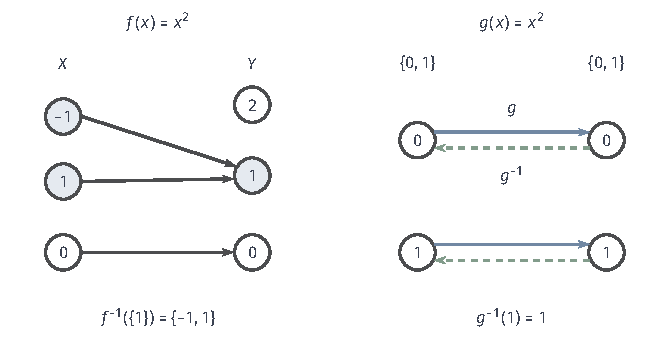
\includegraphics[width=112.0mm]{figures/00-shared/mathematical-preliminaries-upper/01-mathematical-language-combinatorics-analysis-optimization/tikz/prelim-preimage-inverse/figure.pdf}
  \caption{原像与逆映射回答不同问题。左侧$f:\{-1,0,1\}\to\{0,1,2\}$按平方取值，
  标出的$1$有两个原输入，$2$没有原输入；原像$f^{-1}(\{1\})=\{-1,1\}$仍有定义。
  右侧将定义域与陪域都限制为$\{0,1\}$得到双射$g$，实线表示正向求值，虚线表示
  逆映射，因而$g^{-1}(1)=1$是一个元素。两侧均为精确的有限映射。}
  \label{fig:prelim-preimage-inverse}
\end{figure}

\section{索引族}
\label{sec:prelim-indices-sums-recurrences}

三次测验的得分是$1,1,4$，组成集合时只剩$\{1,4\}$，求总分时却要把两个$1$分别计入。
本节用映射给每次出现一个编号，再讨论一族集合的并与交、有限多个数的累计，以及归纳与递归。

\subsection{索引族的定义}
\label{sec:prelim-indexed-sequences}

\paragraph{索引族}
给每次测验一个编号，再为每个编号指定得分，就是一个映射。
\begin{definition}[索引族]
\label{def:prelim-indexed-family}
给定索引集合$I$和对象集合$X$，映射$a:I\to X$也称为以$I$为索引的\term{索引族}（indexed family），
把$a(i)$记作$a_i$，整个族记作$(a_i)_{i\in I}$。$i$称为指标，$a_i$称为指标$i$对应的对象。
\end{definition}
测验得分写成$a_1=1$、$a_2=1$、$a_3=4$。不同指标可以对应相同的对象，所以索引族与取值集合$\{a_i:i\in I\}=\{1,4\}$不同：
前者保留每一次出现，后者只记录出现过哪些值。

\paragraph{序列}
按正整数顺序索引的族称为序列（sequence）：只取$1,\ldots,n$时是有限序列，取全部正整数时是无限序列；
取值为实数的序列称为数列，例如$(1/n)_{n\geq1}$。从$0$开始编号时写$(a_n)_{n\geq0}$。
记录逐步更新的结果时，把第$t$步的结果记作$a^{(t)}$，用带括号的上标表示步数，以区别于幂$a^t$。

\paragraph{二维索引族与集合族}
两个指标共同指定一个对象时，得到二维索引族$(a_{i,j})_{(i,j)\in I\times J}$。
例如$a_{i,j}=3(i-1)+j$（$i=1,2$，$j=1,2,3$）排成两行$(1,2,3)$与$(4,5,6)$，固定$i$得到一行，固定$j$得到一列。

对象也可以是集合，例如三名学生的选课$(S_i)_{i\in\{1,2,3\}}$。这样的族记录的是每份选课，
不能与全部选课的并混为一谈：$S_1=\{1,2\}$、$S_2=\{2\}$时，并集$\{1,2\}$只记录哪些课程有人选过。

\subsection{集合族的运算}
\label{sec:prelim-indexed-set-operations}

给定全集$U$的子集族$(A_i)_{i\in I}$，“至少属于一个成员”和“属于每个成员”分别定义索引并与索引交：
\begin{equation}
 \begin{aligned}
  \bigcup_{i\in I}A_i&=\{u\in U:\text{存在 }i\in I\text{ 使 }u\in A_i\},\\
  \bigcap_{i\in I}A_i&=\{u\in U:\text{对每个 }i\in I\text{ 都有 }u\in A_i\}.
 \end{aligned}
 \label{eq:sets-indexed-union-intersection}
\end{equation}
$I=\{1,2\}$时回到$A_1\cup A_2$与$A_1\cap A_2$；$I=\mathbb N_+$时也写成$\bigcup_{n=1}^\infty A_n$与$\bigcap_{n=1}^\infty A_n$。

索引集为空时，“存在$i$”无法满足，“对每个$i$”则无从违反。所以按定义，空族的并是空集，空族的交是全集$U$；
后者说明索引交必须在指定的全集中讨论。

两个集合的分配律与De Morgan律都推广到索引族，证明仍是逐个元素核对成员条件。对任一$B\subseteq U$，
\begin{equation}
 \begin{aligned}
  B\cap\bigcup_{i\in I}A_i&=\bigcup_{i\in I}(B\cap A_i),\\
  B\cup\bigcap_{i\in I}A_i&=\bigcap_{i\in I}(B\cup A_i).
 \end{aligned}
 \label{eq:sets-distributive-families}
\end{equation}
以第一式为例：$u$属于左边，当且仅当$u\in B$并且存在$i$使$u\in A_i$，也就是存在$i$使$u\in B\cap A_i$。

De Morgan律对任意索引族同样成立：
\begin{equation}
 \begin{aligned}
  \Bigl(\bigcup_{i\in I}A_i\Bigr)^{\mathrm c}&=\bigcap_{i\in I}A_i^{\mathrm c},\\
  \Bigl(\bigcap_{i\in I}A_i\Bigr)^{\mathrm c}&=\bigcup_{i\in I}A_i^{\mathrm c},
 \end{aligned}
 \label{eq:prelim-de-morgan-families}
\end{equation}
证明与定理~\ref{thm:sets-de-morgan}相同：不存在$i$使$u\in A_i$，就是对每个$i$都有$u\in A_i^{\mathrm c}$。

\begin{example}[区间族的无限并与无限交]
\label{ex:sets-interval-family-limits}
在$U=[0,1]$中取递增族$A_n=[1/n,1]$与递减族$B_n=[0,1/n)$，则
\[
 \bigcup_{n\geq1}A_n=(0,1],\qquad \bigcap_{n\geq1}B_n=\{0\}.
\]
对第一式，每个$x>0$在$n\geq1/x$时属于$A_n$，而$0$不属于任何$A_n$。
对第二式，$0$属于每个$B_n$，而每个$x>0$在$n>1/x$时不属于$B_n$。
\end{example}
成员都是区间，无限并却缺了端点，无限交只剩一个点；后面测量集合时还会遇到这类现象。

\subsection{有限累计}
\label{sec:prelim-finite-sums-products}

\paragraph{有限和与有限积}
对$n\geq1$个数$a_1,\ldots,a_n$，记
\[
 \sum_{i=1}^{n}a_i=a_1+\cdots+a_n,\qquad \prod_{i=1}^{n}a_i=a_1\cdots a_n.
\]
这两个记号只是有限次运算的缩写，可以逐项规定：
\[
 \sum_{i=1}^{n+1}a_i=\sum_{i=1}^na_i+a_{n+1},
\]
积同理。逐项规定需要起点，约定空和为$0$、空积为$1$：
\[
 \sum_{i\in\varnothing}a_i=0,\qquad \prod_{i\in\varnothing}a_i=1,
\]
这样把一组项拆成两部分分别汇总时，即使一部分为空，结果也不变。
对有限索引集合$I$，也写$\sum_{i\in I}a_i$与$\prod_{i\in I}a_i$；这些记号在整数、有理数、实数中含义相同。

\paragraph{索引与有限换序}
求和变量的名称不影响结果：$\sum_{i=1}^na_i=\sum_{k=1}^na_k$，这里的$i$称为\term{哑索引}（dummy index）。
自由索引则留在结果中：在$b_j=\sum_{i=1}^{n}x_{i,j}$中，$j$须固定才知道汇总的是哪一列，
所以可以把$i$改为$k$，却不能只改右边的$j$，也不能把$i$改名为已占用的$j$。
平移哑索引时，范围要随之改写：$\sum_{n=1}^{N}b_{n+1}=\sum_{m=2}^{N+1}b_m$。

平移是一种重新编号。一般地，若$\sigma:J\to I$是有限索引集合之间的双射，则
\begin{equation}
 \sum_{j\in J}a_{\sigma(j)}=\sum_{i\in I}a_i,
 \label{eq:prelim-reindexing-sum}
\end{equation}
因为$\sigma$是双射，左边恰好把每个$a_i$计入一次，再由加法的交换律与结合律，改变相加的次序不改变结果；积同理。
前面写$\sum_{i\in I}a_i$而不规定$I$中元素的次序，依据的正是这一点。

若重新编号的映射不是双射，例如把两个指标都送到同一个$i$，$a_i$就被计入两次。因此改变索引时，要核对每一项的出现次数保持不变。

由加法、乘法的交换律、结合律与分配律，有限和满足线性关系
\begin{equation}
 \sum_{i=1}^{n}(\alpha u_i+\beta v_i)=\alpha\sum_{i=1}^{n}u_i+\beta\sum_{i=1}^{n}v_i.
 \label{eq:prelim-sum-linearity}
\end{equation}
有限积则满足逐项相乘与提出常数两条规则：
\[
 \begin{aligned}
  \prod_{i=1}^n(a_ib_i)&=\Bigl(\prod_{i=1}^na_i\Bigr)\Bigl(\prod_{i=1}^nb_i\Bigr),\\
  \prod_{i=1}^n(ca_i)&=c^n\prod_{i=1}^na_i.
 \end{aligned}
\]
积没有线性关系，例如$(1+2)(3+4)\neq1\cdot3+2\cdot4$。

结合平移与线性关系得到裂项求和：
\begin{equation}
 \begin{aligned}
  \sum_{n=1}^N(b_{n+1}-b_n)&=\sum_{m=2}^{N+1}b_m-\sum_{n=1}^{N}b_n\\
  &=b_{N+1}-b_1.
 \end{aligned}
 \label{eq:prelim-telescoping-sum}
\end{equation}
例如由$\frac1{n(n+1)}=\frac1n-\frac1{n+1}$，取$b_n=-\frac1n$，得到
\[
 \sum_{n=1}^N\frac1{n(n+1)}=1-\frac1{N+1}.
\]

对二维有限数组$(a_{i,j})$，$i=1,\ldots,n$，$j=1,\ldots,d$，按行汇总与按列汇总相等：
\begin{equation}
 \sum_{i=1}^{n}\sum_{j=1}^{d}a_{i,j}=\sum_{j=1}^{d}\sum_{i=1}^{n}a_{i,j},
 \label{eq:prelim-sum-interchange}
\end{equation}
因为两边都把每个索引对恰好计入一次。

内层范围依赖外层索引时，换序要重写范围，使遍历的仍是同一批索引对：
\begin{equation}
 \sum_{i=1}^{n}\sum_{j=1}^{i}a_{i,j}=\sum_{j=1}^{n}\sum_{i=j}^{n}a_{i,j},
 \label{eq:prelim-triangular-sum}
\end{equation}
两边都恰好遍历满足$1\leq j\leq i\leq n$的$(i,j)$；若把右边内层误写成$i=1,\ldots,n$，就会多算$j>i$的项。
这些换序依赖项数有限；无限多项的和要先用极限定义，不能由有限情形直接推广。

\subsection{数学归纳与递归}
\label{sec:prelim-recurrence-unrolling}

\paragraph{数学归纳}
\term{数学归纳法}（mathematical induction）给出证明方法：
要证明关于$N=0,1,2,\ldots$的命题$P(N)$全部成立，只需证明$P(0)$成立（归纳基础），
以及对每个$N\geq0$，由$P(N)$能推出$P(N+1)$（归纳步）；归纳步中假定成立的$P(N)$称为归纳假设。

\begin{example}[前$N$个正整数之和]
\label{ex:sets-induction-arithmetic-sum}
令$S_N=1+2+\cdots+N$并约定$S_0=0$，我们用归纳法验证
\[
 S_N=\frac{N(N+1)}2,\qquad N\geq0.
\]
$N=0$时两边都为零。若公式对$N$成立，则
\[
 S_{N+1}=S_N+(N+1)=\frac{N(N+1)}2+(N+1)=\frac{(N+1)(N+2)}2.
\]
因此公式也对$N+1$成立，由归纳法对每个$N\geq0$成立。
\end{example}

同样的方法也能验证有限几何和。令$G_N=\sum_{n=0}^N\rho^n$。对$\rho\neq1$，先计算$G_0=1$、$G_1=1+\rho$，再猜测
\begin{equation}
 \sum_{n=0}^{N}\rho^n=\frac{1-\rho^{N+1}}{1-\rho},\qquad
 \sum_{n=0}^{N}1^n=N+1.
 \label{eq:prelim-finite-geometric-sum}
\end{equation}
第一式在$N=0$时成立，两边都是$1$。若它对$N$成立，加入下一项$\rho^{N+1}$并通分，得到
\[
 \begin{aligned}
  G_{N+1}&=\frac{1-\rho^{N+1}}{1-\rho}+\rho^{N+1}
  =\frac{1-\rho^{N+1}+\rho^{N+1}-\rho^{N+2}}{1-\rho}\\
  &=\frac{1-\rho^{N+2}}{1-\rho},
 \end{aligned}
\]
这正是$N+1$时的公式。

第二式对应$\rho=1$，这时第一式的分母为零而不能使用，和式则是$N+1$个$1$相加。

有时证明$P(N+1)$要用到此前的全部命题。强归纳法规定：若$P(0)$成立，并且对每个$N\geq0$，
由$P(0),\ldots,P(N)$全部成立能推出$P(N+1)$，则$P(N)$对一切$N$成立；把命题换成“$P(0),\ldots,P(N)$都成立”，它就回到普通归纳。
\begin{example}[整数分解为素数之积]
\label{ex:sets-strong-induction-primes}
要证明每个大于$1$的整数$m$都是素数之积（单个素数也算一个积）。对$m=2,3,\ldots$用强归纳：设结论对$2,\ldots,m-1$都成立。
若$m$是素数，结论成立；否则$m=ab$，$1<a,b<m$。$a,b$都比$m$小，由归纳假设都是素数之积，把两个乘积接起来，$m$也是素数之积。

这里$a,b$可以是$m-1$以前的任何数，而不只是$m-1$，所以需要强归纳。
\end{example}

\paragraph{递归}
给定集合$X$、初值$x_0\in X$与更新映射$T:X\to X$，规定
\begin{equation}
 x_{t+1}=T(x_t),\qquad t=0,1,2,\ldots,
 \label{eq:prelim-recurrence}
\end{equation}
这种用已有的项确定下一项的定义方式称为\term{递推}（recurrence），也称递归定义；有限和的逐项规定就是一例。

这样的规定看似理所当然，但“无限多项都已确定”需要论证，因为我们每次只能写出有限多项。
论证的办法是只处理有限段，再用归纳把它们拼起来。
称满足$y_0=x_0$且$y_{k+1}=T(y_k)$（$0\leq k<n$）的有限组$(y_0,\ldots,y_n)$为长度$n+1$的初段。

对$n$归纳可知，每个长度的初段恰有一个：长度$1$的初段只能是$(x_0)$；若长度$n+1$的初段唯一，
它后面只能接上$T(y_n)$，所以长度$n+2$的初段也唯一，并且它的前$n+1$项就是长度$n+1$的初段。

令$x_n$为长度$n+1$的初段的末项，就得到满足递推的序列$(x_n)_{n\geq0}$。
反过来，任何满足递推的序列的前$n+1$项都是长度$n+1$的初段，因而与$x_0,\ldots,x_n$相同。所以递推确定了唯一的序列。

递推用来定义序列，归纳法则可以验证序列的性质。
\begin{example}[折半递推的通项]
\label{ex:sets-halving-recurrence}
取初值$x_0=8$和更新规则$x_{t+1}=x_t/2$，
逐项得到$8,4,2,1,\ldots$，由此猜测
\[
 x_t=\frac{8}{2^t}.
\]
$t=0$时公式成立。若某一步满足这一公式，代入更新规则得
\[
 x_{t+1}=\frac{x_t}{2}=\frac{8}{2^{t+1}},
\]
公式对下一步也成立。由归纳法，通项公式对每个非负整数$t$成立。
\end{example}

更一般地，等比递推
\begin{equation}
 e^{(t+1)}=\rho e^{(t)},\qquad e^{(0)}=e_0
 \label{eq:prelim-geometric-recurrence}
\end{equation}
由同样的归纳步骤得到通项
\begin{equation}
 e^{(t)}=\rho^te_0,\qquad t\geq0.
 \label{eq:prelim-geometric-recurrence-solution}
\end{equation}
它在步数无限增大时的行为将在第~\ref{chap:limits-continuity}章讨论。

\section{本章小结}
\label{sec:prelim-sets-functions-summary}

回到章首的选课记录。“有哪些课程”由集合回答：集合只由元素决定，集合相等用双向包含证明，
交换、结合、分配律与De Morgan律都能逐个元素核对，差集则没有交换律和结合律。
幂集把“一名学生的全部选课”当作一个对象，笛卡尔积则记录有次序、可重复的多次选择。

“谁与谁有联系”由关系回答，关系就是笛卡尔积的子集。等价关系与划分是同一结构的两种写法，
商集把每一类当作新对象，在商集上定义运算或映射时，结果必须与代表元的选取无关。
偏序允许对象互不可比，所以最小元与极小元要分别判断；界与确界可以落在集合之外，确界属于集合时才是最值，而一般偏序并不保证确界存在。

“怎样把一个对象对应到另一个对象”由映射回答，映射要求每个输入恰有一个输出。原像保持并、交与补；
像保持并，保持交则需要单射。单射、满射与双射依赖源集和目标集的选取，双射恰好是具有双侧逆映射的映射；
逆映射作用于元素，只对双射存在，原像作用于集合，对任何映射都有定义。

“怎样编号并累计”由索引族回答。索引族保留每次出现，集合族的并、交、分配律与De Morgan律对任意索引集成立；
有限和与有限积可以重新编号和换序，条件是每一项仍恰好计入一次，而无限多项的和要另用极限定义。
递推定义逐项生成的对象，归纳证明关于全部自然数的命题，两者常配合使用。

全章要分清对象本身与它的编号、等价类与代表元、映射与表示它的规则表达式。
下一章用双射把有限集合与$\{1,\ldots,n\}$配对，借助分类、分步、对应和递推计数；
第~\ref{chap:cardinality}章再用单射和双射比较无限集合的大小。实数的确界、实值函数的运算和极限从第~\ref{chap:real-complex-functions}章开始讨论。

\chapter{计数}
\label{chap:combinatorics}
\label{chap:counting}

从四门课中任选一些，共有多少种选法？从四名学生中选出组长和记录员，又有多少种安排？
对象稍多时，逐一列举既费力又容易重复或遗漏。本章研究怎样不逐一列举而算出有限集合的元素个数。

计数前先要确定什么算一个结果。从四个对象中依次取两个，$(1,3)$与$(3,1)$是不同的有序记录；
若只记录选中了哪些对象，它们都是子集$\{1,3\}$。记录方式不同，结果数也不同。
所以每个计数问题都要先说清：结果是有序组还是集合，是否允许重复，各部分有没有名称，以及有哪些限制条件。

“数一数”本身也要说清含义。借助第~\ref{chap:sets-relations-maps}章的双射，有限集合$A$有$n$个元素，是说存在双射$\{1,\ldots,n\}\to A$，
即能把$A$的元素恰好编号为$1,\ldots,n$；空集对应$n=0$。$A$的元素个数记为$|A|$。

有了这个定义，计数的基本手段都可以归结为映射与集合运算：把结果集合换成与它一一对应、较容易数的集合，
把结果分成互不重叠的几类，或把每个结果拆成依次进行的几步选择。第一节由此推出加法规则与乘法规则。
第二节把它们用于“是否记录次序、是否允许重复”这两个最常见的区分，得到排列数、组合数与二项式展开。
第三节处理加法规则不能直接使用的两种情形：类别相互重叠，或问题能化为更小的同类问题。

以下记$V=\{1,\ldots,n\}$，其中$n\geq0$。

\section{分类和分步计数}
\label{sec:comb-families-counting}
\label{sec:comb-finite-counting}
\label{sec:comb-decomposition-counting}
\label{sec:comb-classification-products}
\label{sec:comb-classification-counting}

本节先说明双射为什么能用来计数，以及元素个数为什么不依赖编号方式；再由编号的拼接得到加法规则，由按第一步分类得到乘法规则。

\paragraph{双射与计数}
数出有限集合$A$有$n$个元素，就是给出编号双射$g:\{1,\ldots,n\}\to A$。若另有双射$f:A\to B$，
则$f\circ g$把$B$的元素也恰好编号为$1,\ldots,n$。所以两个有限集合之间存在双射时，元素个数相同。
这给出计数的第一种手段：要数一个集合，可以改数一个与它一一对应、但更容易数的集合。

使用元素个数之前还要确认，同一个集合不会数出两个不同的个数。若$A$既能编号为$1,\ldots,m$又能编号为$1,\ldots,n$，
把一种编号的逆与另一种复合，就得到双射$\{1,\ldots,m\}\to\{1,\ldots,n\}$。
所以只需证明：若$h:\{1,\ldots,m\}\to\{1,\ldots,n\}$是双射，则$m=n$。

对$n$归纳。$n=0$时目标集为空，源集中若有元素便无处可去，所以源集也为空，即$m=0$。

$n\geq1$时目标集非空，满射要求源集非空，即$m\geq1$。设$h(j)=n$，交换$h$在$j$与$m$处的取值，得到仍为双射且把$m$送到$n$的映射；
把它限制到$\{1,\ldots,m-1\}$，得到到$\{1,\ldots,n-1\}$的双射，由归纳假设$m-1=n-1$。

\paragraph{加法规则}
若有限集合$A_1,\ldots,A_r$两两不交，则
\begin{equation}
 \Bigl|\bigcup_{i=1}^r A_i\Bigr|=\sum_{i=1}^r|A_i|,
 \label{eq:comb-addition-rule}
\end{equation}
这称为计数的加法规则。它来自编号的拼接：先给$A_1$的元素编号$1,\ldots,|A_1|$，再从$|A_1|+1$起接着给$A_2$编号，依此类推；
两两不交保证没有元素被编号两次。

使用时要检查各类覆盖全部结果且两两不交；类别重叠的情形留给第~\ref{sec:comb-overlap-counting}节的容斥原理。

由加法规则，若$B\subsetneq A$都是有限集合，则$A$是不交的$B$与$A\setminus B$之并，后者非空，所以
\[
 |A|=|B|+|A\setminus B|>|B|,
\]
即有限集合的真子集元素更少。第~\ref{chap:cardinality}章将看到，这一点对无限集合不再成立。

加法规则的一个推论是\term{抽屉原理}（pigeonhole principle）：把$m$个对象放进$k$个位置，若每个位置至多一个对象，
按位置分类得$m\leq k$；因此$m>k$时必有某个位置容纳至少两个对象。例如任选$13$人，必有两人同月出生。
换句话说，$m>k$时从$m$元集到$k$元集的映射都不是单射。

\paragraph{乘法规则}
\phantomsection
\label{sec:comb-stepwise-counting}
对有限集合$A_1,\ldots,A_r$，
\begin{equation}
 |A_1\times\cdots\times A_r|=\prod_{i=1}^r|A_i|,
 \label{eq:comb-multiplication-rule}
\end{equation}
这称为计数的乘法规则。$r=2$时，按第一个位置的取值把$A_1\times A_2$分成$|A_1|$类，
第$a$类$\{a\}\times A_2$与$A_2$之间有双射$(a,b)\mapsto b$，每类都有$|A_2|$个元素，由加法规则得$|A_1|\cdot|A_2|$。

一般的$r$对位置个数归纳。$A_1\times\cdots\times A_{r+1}$与$(A_1\times\cdots\times A_r)\times A_{r+1}$之间有双射
\[
 ((a_1,\ldots,a_r),a_{r+1})\mapsto(a_1,\ldots,a_{r+1}),
\]
所以前者的元素个数是$|A_1\times\cdots\times A_r|\cdot|A_{r+1}|$，再用归纳假设。

例如第一位取$a,b$之一、第二位取$1,2,3$之一，共有$2\times3=6$个结果，逐一列出如下：
\[
 (a,1),\ (a,2),\ (a,3),\ (b,1),\ (b,2),\ (b,3).
\]
长度为$n$的零一记录组成$\{0,1\}^n$，共$2^n$条。

分步选择中，后一步的选项常依赖前一步，例如先选组长、再从其余人中选记录员，记录员的人选随组长而变。
这时结果集合不再是笛卡尔积，但只要第$i$步在每种已有记录之后都恰有$n_i$个选项，完整记录数仍是$\prod_in_i$。
证明对步数归纳：按第一步的选择分成$n_1$类，由归纳假设每类都有$\prod_{i\geq2}n_i$个记录，再用加法规则。

所以乘法规则要求的是每步选项的个数固定，选项的内容可以变化。若个数也随前一步改变，就先按前一步分类，再在各类中分别用乘法规则并相加。
\begin{example}[辅修选项随主修变化]
\label{ex:comb-major-minor}
从四门课中选一门主修，主修课程$1$时只能从课程$2,3$中选辅修，
否则可从其余三门中选，完整记录数是$1\times2+3\times3=11$。
\end{example}

\section{排列与组合}
\label{sec:comb-permutation-combination-counts}
\label{sec:comb-subset-partition-counts}

选取若干对象时，可以记录它们所在的位置，也可以只记录选中了谁。先按位置计数，再把只是位置不同的记录归为一类，
就能联系这两类问题；不限选取个数或二分对象时，则可以借助零一记录。

\paragraph{排列数}
设$0\leq k\leq n$。从$n$个不同对象中取出$k$个依次放在$k$个位置上且不重复，所得有序$k$元组称为排列，个数记为$P(n,k)$。
各位置依次有$n,n-1,\ldots,n-k+1$种选择，由乘法规则
\begin{equation}
 P(n,k)=\prod_{i=0}^{k-1}(n-i)=n(n-1)\cdots(n-k+1),
 \label{eq:comb-permutation-count}
\end{equation}
$k=0$时为空积$1$，对应唯一的空排列。例如从四人中选组长和记录员有$P(4,2)=12$种安排。

$n(n-1)\cdots1$记作$n!$，称为$n$的\term{阶乘}（factorial），约定$0!=1$，于是$P(n,k)=n!/(n-k)!$。

若允许重复选取，每个位置都有$n$个选项，有序记录数是$n^k$；例如连续两天从三道菜中各选一道，允许重复时有$9$种，不允许时有$6$种。

\paragraph{组合数}
若只记录选中的对象，结果是一个$k$元子集，称为组合，个数记为$\binom nk$，读作“$n$选$k$”。
每个排列确定一个$k$元子集，每个$k$元子集又恰好对应$k!$个排列，所以全部排列按子集分成$\binom nk$类，每类$k!$个，
加法规则给出$P(n,k)=\binom nk k!$，即
\begin{equation}
 \binom nk=\frac{P(n,k)}{k!}=\frac{n!}{k!(n-k)!},\qquad 0\leq k\leq n.
 \label{eq:prelim-binomial-coefficient}
\end{equation}
例如十二种组长—记录员安排中每个二人小组恰好出现两次，所以二人小组有$6$个。

先把人数缩小到三人，图~\ref{fig:v1-permutations-to-subsets}显示“除以$2!$”是在合并哪些记录；每个无序结果都恰好对应两条有序记录。
\begin{figure}[!htbp]
 \centering
 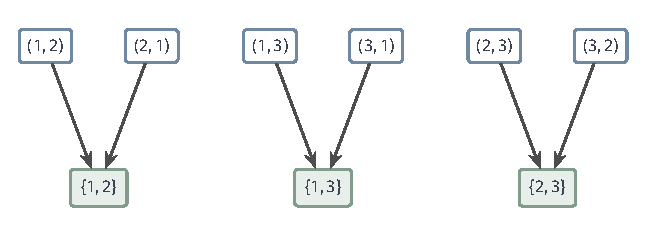
\includegraphics[width=112mm]{figures/01-sets-and-univariate-calculus/01-sets/tikz/permutations-to-subsets/figure.pdf}
 \caption{从$\{1,2,3\}$中选两人的有序与无序记录。箭头表示忘去次序，六个有序对分成三组，每组映到同一个二元子集。这是$P(3,2)/2!=\binom32=3$的具体对应。}
 \label{fig:v1-permutations-to-subsets}
\end{figure}



取补集给出$k$元子集与$(n-k)$元子集的双射，所以$\binom nk=\binom n{n-k}$；$\binom n0=\binom nn=1$分别对应空集与全体，
并约定$k<0$或$k>n$时$\binom nk=0$。允许重复的无序选择则不能直接套用组合数。

从$n$种水果中挑$k$个、同种不加区分，结果由各种的个数$(m_1,\ldots,m_n)$决定，$\sum_im_i=k$。
依次写$m_1$个星号、一条竖线、$m_2$个星号……，得到$k$个星号与$n-1$条竖线排成的一行，二者一一对应。
所以结果数是从$n+k-1$个位置中选出星号位置的方法数：
\begin{equation}
 \binom{n+k-1}{k}.
 \label{eq:comb-multiset-count}
\end{equation}
例如从三种水果中挑两个，有$\binom42=6$种。

图~\ref{fig:v1-stars-and-bars}逐一对应三种水果中挑两个的六种结果。相邻分隔线表示某一种没有被选中，因而零个的情形也自动包含在编码中。
\begin{figure}[!htbp]
 \centering
 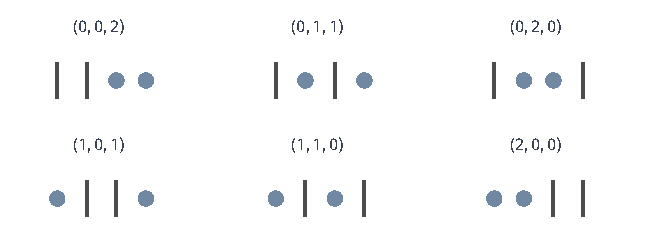
\includegraphics[width=112mm]{figures/01-sets-and-univariate-calculus/01-sets/tikz/stars-and-bars/figure.pdf}
 \caption{星号竖线法的六种编码。每个蓝点代替一个星号，两条竖线把这一行分成三段，各段蓝点的个数依次是上方的$(m_1,m_2,m_3)$。共有四个位置，其中任选两个放星号；点与线均为计数符号。}
 \label{fig:v1-stars-and-bars}
\end{figure}



\paragraph{幂集与组合恒等式}
\phantomsection
\label{sec:comb-ordered-unordered}
每个子集$S\subseteq V$对应一条零一记录$(z_1,\ldots,z_n)$，$z_i=1$当且仅当$i\in S$；这是$\mathcal P(V)$到$\{0,1\}^n$的双射，所以
\begin{equation}
 |\mathcal P(V)|=2^n.
 \label{eq:comb-power-set-count}
\end{equation}
另一方面，按大小把子集分成$0,1,\ldots,n$元子集，加法规则给出子集总数$\sum_k\binom nk$。对同一集合的这两种计数称为双重计数，它给出
\begin{equation}
 \sum_{k=0}^n\binom nk=2^n.
 \label{eq:comb-binomial-sum}
\end{equation}

\paragraph{二项式展开}
组合数之所以又称二项式系数，是因为它们恰好是$(x+y)^n$展开后的系数。展开$(x+y)^2=x^2+2xy+y^2$时，
$xy$的系数$2$来自两种取法：从第一个因子取$x$、第二个取$y$，或者反过来。一般情形同样是在数“取法”。
\begin{theorem}[二项式定理]
\label{thm:comb-binomial-theorem}
对任意实数$x,y$与整数$n\geq0$，
\begin{equation}
 (x+y)^n=\sum_{k=0}^n\binom nk x^ky^{n-k}.
 \label{eq:comb-binomial-theorem}
\end{equation}
\end{theorem}
\begin{proof}
把$(x+y)^n$写成$n$个因子$(x+y)$之积。反复使用分配律，乘积展开为若干项之和：每一项从每个因子中取出$x$或$y$之一相乘，
不同的取法给出不同的项，而且每种取法恰好出现一次。对因子个数归纳可以核对这一点：
若前$n-1$个因子之积已展开为各种取法之和，再乘上$(x+y)$，由分配律，每种旧取法分成“第$n$个因子取$x$”和“取$y$”两种新取法。

每种取法对应一条零一记录$\bm z\in\{0,1\}^n$，$z_i=1$表示第$i$个因子取$x$；它也对应子集$S=\{i:z_i=1\}\subseteq V$。
取法$S$给出的项是$x^{|S|}y^{n-|S|}$。按$|S|=k$把全部取法分类，第$k$类有$\binom nk$种取法，每种都给出$x^ky^{n-k}$，
合并同类项即得结论。
\end{proof}
取$x=y=1$就回到上面的$\sum_k\binom nk=2^n$：两种计数说的都是$V$的全部子集，二项式定理只是给每个子集记上了“权重”$x^{|S|}y^{n-|S|}$。

交错和$\sum_k(-1)^k\binom nk$对应$x=-1$、$y=1$，由二项式定理等于$0^n$：$n\geq1$时为$0$，$n=0$时是空积$0^0=1$。

这一交错和也可以直接解释为偶数大小子集数减去奇数大小子集数，并用配对说明两者相等。当$n\geq1$时，固定元素$n$，
对每个子集作“含$n$则删去、不含则加入”的改动；它是$\mathcal P(V)$到自身的双射，并把子集大小改变$1$，
因而把偶数大小的子集一一配对到奇数大小的子集，所以
\begin{equation}
 \sum_{k=0}^n(-1)^k\binom nk=0,\qquad n\geq1.
 \label{eq:comb-alternating-subset-count}
\end{equation}
配对的说法直接显示了正负项怎样两两抵消；下一节的容斥原理就依靠这一抵消。

\paragraph{二分划分}
把一批对象分成两组时，除了次序和重复，还要问两组有没有名称。若两侧有名称，例如“已选”和“未选”，
结果$(S,V\setminus S)$由$S$唯一确定，共$2^n$个。

若两侧没有名称，例如把$n$人分成两队而不区分队名，结果是$\{S,V\setminus S\}$。$n\geq1$时$S\neq V\setminus S$，
每个无名称结果恰有$(S,V\setminus S)$与$(V\setminus S,S)$两个有名称表示，所以无名称结果有$2^{n-1}$个。
这与组合数的推导相同：每个结果被记录同样多次时，用记录数除以重复次数。

要求两侧非空时，去掉$(\varnothing,V)$与$(V,\varnothing)$，得到$2^n-2$个有名称结果与$2^{n-1}-1$个无名称结果。
$n=0$时只有$(\varnothing,\varnothing)$，两侧相同，每个结果只有一个表示，所以不能用除以$2$的公式。

\section{重叠计数与递推计数}
\label{sec:comb-overlap-counting}
\label{sec:comb-inclusion-mobius}

本节处理加法规则不能直接使用的两种情形：类别重叠时用交集校正重复计数；问题能化为更小的同类问题时建立递推。

\paragraph{容斥原理}
设$A=\{1,2,3,4\}$、$B=\{3,4,5\}$。$|A|+|B|=7$把公共元素$3,4$各数了两次，减去交集得$|A\cup B|=7-2=5$。
一般地，把并集分成$A\setminus B$、$A\cap B$、$B\setminus A$三个不交部分并用加法规则，得到
\[
 |A\cup B|=|A|+|B|-|A\cap B|.
\]
图~\ref{fig:comb-inclusion-exclusion-overlap}显示了被多数一次的公共区域。
\begin{figure}[htbp]
  \centering
  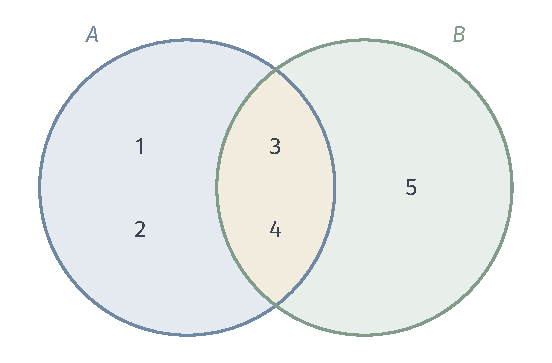
\includegraphics[width=90mm]{figures/00-shared/mathematical-preliminaries-upper/01-mathematical-language-combinatorics-analysis-optimization/tikz/inclusion-exclusion-overlap.pdf}
  \caption{两个有限集合的重叠计数。$A=\{1,2,3,4\}$，$B=\{3,4,5\}$；仅属于$A$的区域放入$1,2$，公共区域放入$3,4$，仅属于$B$的区域放入$5$。把两圈元素个数相加时，公共区域被数两次，减去一次后得到并集中的五个不同元素。}
  \label{fig:comb-inclusion-exclusion-overlap}
\end{figure}

对三个集合逐元素检查：恰属于两个集合的元素先计两次、再减一次；同属三者的元素先计三次、减三次，还需加回一次。所以
\[
 \begin{aligned}
  |A\cup B\cup C|&=|A|+|B|+|C|\\
  &\quad-|A\cap B|-|A\cap C|-|B\cap C|\\
  &\quad+|A\cap B\cap C|.
 \end{aligned}
\]
\term{容斥原理}（inclusion--exclusion principle）把这种交替加减推广到任意有限个集合。
\begin{theorem}[有限容斥原理]
\label{thm:comb-inclusion-exclusion}
设$A_1,\ldots,A_m$是有限集合。则
\begin{equation}
  \Bigl|\bigcup_{i=1}^{m}A_i\Bigr|
  =\sum_{\varnothing\neq I\subseteq\{1,\ldots,m\}}(-1)^{|I|+1}\Bigl|\bigcap_{i\in I}A_i\Bigr|.
  \label{eq:comb-inclusion-exclusion}
\end{equation}
\end{theorem}
\begin{proof}
左侧把并集的每个元素恰计一次。右侧的每一项$|\bigcap_{i\in I}A_i|$也是在数元素，可以改为逐个元素统计：
元素$x$在右侧的总系数，是它所属的那些交集所带符号$(-1)^{|I|+1}$之和。只需证明这一总系数对并集中的元素为$1$，对其余元素为$0$。
设$x$恰属于$r$个集合，其下标组成$J$；$x$属于$\bigcap_{i\in I}A_i$当且仅当$I\subseteq J$。
$r=0$时$x$不在并集中，两侧都不计入。$r\geq1$时，大小为$k$的$I\subseteq J$有$\binom rk$个，所以$x$的总系数为
\[
 \sum_{k=1}^r(-1)^{k+1}\binom rk=-\Bigl(\sum_{k=0}^r(-1)^k\binom rk-1\Bigr)=1,
\]
最后一步用式~\eqref{eq:comb-alternating-subset-count}。所以两侧相等。
\end{proof}

\paragraph{补集计数}
有多条限制时，可以先数违反限制的结果，再从总数中减去。
\begin{example}[带限制的选课方案]
\label{ex:comb-constrained-course-selection}
四门课的选法记作$\bm z\in\{0,1\}^4$，其中$z_i=1$表示选第$i$门。
规则是：课程$1,2$恰选一门；选课程$3$就必须选课程$1$；选课程$4$就必须在课程$2,3$中至少选一门。违反各条规则的选法分别组成
\[
 \begin{aligned}
 A_1&=\{\bm z:z_1=z_2\},\\
 A_2&=\{\bm z:z_3=1,\ z_1=0\},\\
 A_3&=\{\bm z:z_4=1,\ z_2=z_3=0\}.
 \end{aligned}
\]
由De Morgan律，合法选法组成$(A_1\cup A_2\cup A_3)^{\mathrm c}$，个数为$16-|A_1\cup A_2\cup A_3|$。

各集合只固定了部分坐标，其余坐标任取，用乘法规则读出
\[
 |A_1|=8,\qquad |A_2|=4,\qquad |A_3|=2.
\]
两两的交集逐个检查：$A_1\cap A_2$要求$z_1=z_2=0$、$z_3=1$，有$2$个元素；
$A_1\cap A_3$只含$(0,0,0,1)$；$A_2\cap A_3$要求$z_3$既为$1$又为$0$，是空集，因而三者之交也是空集。

由容斥原理，违规选法的个数是
\[
 8+4+2-2-1-0+0=11,
\]
合法选法为$16-11=5$种，对应的课程集合族是
\[
 \mathcal C_0=\bigl\{\{1\},\{1,3\},\{1,3,4\},\{2\},\{2,4\}\bigr\}.
\]
直接分支计数也得到同样的五种：$z_1=1$时$z_3$任取、$z_4=1$须$z_3=1$，共三种；$z_2=1$时$z_3=0$、$z_4$任取，共两种。
\end{example}

\paragraph{递推计数}
固定元素$n$，把$V$的$k$元子集分成不含$n$与含$n$两类，分别有$\binom{n-1}k$与$\binom{n-1}{k-1}$个，所以
\[
 \binom nk=\binom{n-1}k+\binom{n-1}{k-1},\qquad n\geq1,
\]
称为Pascal恒等式。把它当作递推：令$a_{0,0}=1$，$0\leq k\leq n$以外的$a_{n,k}=0$，并对$n\geq1$规定
\begin{equation}
 a_{n,k}=a_{n-1,k}+a_{n-1,k-1}.
 \label{eq:comb-binomial-recurrence}
\end{equation}
逐行得到$(1)$、$(1,1)$、$(1,2,1)$、$(1,3,3,1)$、$(1,4,6,4,1)$；越界值取零使两端也适用同一规则。
对$n$归纳，并用Pascal恒等式与越界约定，可知$a_{n,k}=\binom nk$。图~\ref{fig:vol1-add-pascal-recurrence}标出了$\binom42=3+3$的来源。
\begin{figure}[!htb]
  \centering
  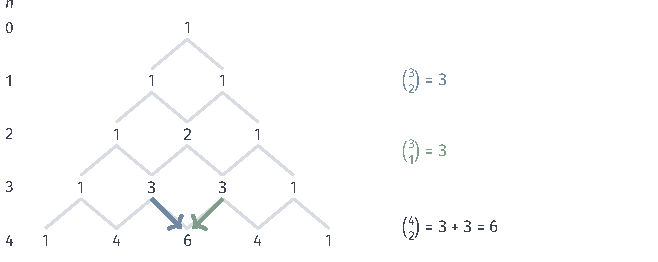
\includegraphics[width=112mm]{figures/00-shared/mathematical-preliminaries-upper/00-shared/tikz/mathematical-language-combinatorics-analysis-optimization-comprehension-additions/pascal-recurrence.pdf}
  \caption{组合数的逐行递推。第$n$行列出$\binom n0,\ldots,\binom nn$；箭头突出$\binom42=\binom32+\binom31=3+3$。两种分类分别从其余三个元素选两个，或先保留固定元素再从其余三个中选一个。网格位置表示递推依赖，不表示子集包含关系。}
  \label{fig:vol1-add-pascal-recurrence}
\end{figure}

一般地，按固定元素、规模或最后一步分类，使每类成为更小的同类问题，就能建立递推。
\begin{example}[不含相邻两个$1$的零一记录]
\label{ex:comb-no-adjacent-ones}
设长度为$n$、不含相邻两个$1$的零一记录个数为$f_n$。按最后一位分类，末位为$0$时前$n-1$位任意合格，
末位为$1$时倒数第二位须为$0$、前$n-2$位任意合格，所以
\[
 f_n=f_{n-1}+f_{n-2},\qquad n\geq2.
\]

初值是$f_0=1$（只有空记录）与$f_1=2$（记录$0$与$1$）。由递推逐项算出$f_2=3$、$f_3=5$、$f_4=8$。

用$n=3$核对：合格记录是$000,001,010,100,101$，恰为五条。
\end{example}
递推式须与初值、适用范围一起写明。这里$n\geq2$的限制不可省略：$n=1$时“前$n-2$位”没有意义，$f_1$只能由直接列举得到。

\paragraph{求解简单递推}
递推本身已能逐项算出答案；若还想得到通项公式，最简单的情形是每一项只依赖前一项。
设$s_n=|\mathcal P(V)|$。按是否含元素$n$分类，不含$n$的子集就是$\{1,\ldots,n-1\}$的子集，含$n$的子集删去$n$后也是，
两类之间有双射$S\mapsto S\cup\{n\}$，所以
\[
 s_n=2s_{n-1},\qquad n\geq1,\qquad s_0=1.
\]
这正是第~\ref{chap:sets-relations-maps}章的等比递推~\eqref{eq:prelim-geometric-recurrence}，取$\rho=2$、初值$1$，由归纳得$s_n=2^n$，与式~\eqref{eq:comb-power-set-count}一致。

若每一步还要加上一个随$n$变化的量，可以先把递推写成差，再用裂项求和。设$t_n$是$V$的非空子集个数。
按是否含$n$分类：不含$n$的非空子集有$t_{n-1}$个；含$n$的子集都非空，删去$n$后是$\{1,\ldots,n-1\}$的任意子集，有$2^{n-1}$个。于是
\[
 t_n-t_{n-1}=2^{n-1},\qquad n\geq1,\qquad t_0=0.
\]
对$n=1,\ldots,N$求和。左边由裂项求和~\eqref{eq:prelim-telescoping-sum}只剩$t_N-t_0$；
右边平移指标后是$2$的前$N$个幂之和，由有限几何和~\eqref{eq:prelim-finite-geometric-sum}（取$\rho=2$）得
\[
 \sum_{m=0}^{N-1}2^m=\frac{1-2^N}{1-2}=2^N-1.
\]
再由$t_0=0$得到
\[
 t_N=2^N-1.
\]

求出通项后要回到计数对象核对：全部子集去掉空集，确实剩$2^N-1$个；$N=2$时非空子集是$\{1\},\{2\},\{1,2\}$，也是三个。
这一步检查的是递推是否数对了对象，而不只是代数运算有没有出错。

\section{本章小结}
\label{sec:comb-summary}

本章回答了怎样不逐一列举而数出有限集合的元素个数。出发点是元素个数的定义：有限集合能被双射编号为$1,\ldots,n$，而且$n$唯一。
由此，双射把难数的集合换成好数的集合；互斥且覆盖全部结果的分类用加法，抽屉原理是其推论；
每步选项个数固定的分步选择用乘法，选项个数随前一步改变时先分类再相加。

计数之前要确定什么算一个结果：是否区分次序、是否允许重复、各部分是否有名称。
每个结果被记录同样多次时，记录数等于结果数乘以重复次数，排列数、组合数与无名称二分划分的公式都由此得到；
允许重复的无序选择则要先换成星号与竖线的记录，再用组合数。
子集与零一记录的双射把组合数、幂集大小和二项式展开连在一起：$(x+y)^n$的展开逐项对应$V$的子集，取特殊值就得到$\sum_k\binom nk=2^n$与交错和为零。

加法规则要求类别互不重叠。类别重叠时，容斥原理按“每个元素的总系数为$1$”校正重复，补集计数则借助De Morgan律把“满足全部限制”改写为“不违反任何一条”。
问题能按固定元素、规模或最后一步化为更小的同类问题时，可以建立递推；递推须连同初值和适用范围写出，求出通项后还要回到计数对象核对。

这些方法都依赖有限集合能被编号到某个$n$为止。对数不到最后一个元素的无限集合，
仍可以问两个集合的元素能否一一配对；第~\ref{chap:cardinality}章用双射和单射回答这一问题。

\chapter{基数}
\label{chap:cardinality}

正整数与正偶数，哪一个更多？正偶数只是正整数的一部分，似乎更少；
可是给每个正整数$n$配上正偶数$2n$，两边的元素又恰好一一配完。
有理数在数轴上处处稠密，那么实数与有理数能否一一配对？
无限集合无法像有限集合那样逐个数完。不过上一章已经看到，有限集合的元素个数本来就是用它与$\{1,\ldots,n\}$之间的双射确定的；
数数只是“一一配对”的一种特殊做法。本章把“能否一一配对”当作比较大小的标准，推广到任意集合。

这一标准需要分三步展开。第一节用双射定义“一样多”，并看到无限集合可以与自己的真子集一样多，所以“部分少于整体”不能再作为依据。
第二节用单射定义“不超过”，要回答两个方向的“不超过”能否推出一样多、基数能否像数一样运算、是否存在最大的基数。
第三节以正整数集为标准研究可数集，整理可数性在哪些构造下保持，并证明有理数可数而实数不可数。

本章依赖第~\ref{chap:sets-relations-maps}章的单射、满射、双射与幂集，以及上一章的元素个数与加法、乘法规则。
例子中用到读者熟悉的数系及其十进制表示，实数的确界与完备性在第~\ref{chap:real-complex-functions}章建立。

\section{等势与基数的定义}
\label{sec:comb-cardinality}
\label{sec:comb-equinumerosity-cardinality}

\paragraph{等势与基数}
对任意两个集合，即使数不出个数，也可以问能否把两边的元素恰好一一配完。若存在双射$f:A\to B$，就称集合$A$与$B$\term{等势}（equinumerous）。

等势具有三条性质：
\begin{enumerate}
\item 恒等映射$\operatorname{id}_A$说明$A$与自身等势（自反）；
\item 双射的逆映射仍是双射，所以$A$与$B$等势时$B$与$A$也等势（对称）；
\item 双射的复合仍是双射，所以$A$与$B$、$B$与$C$等势时$A$与$C$等势（传递）。
\end{enumerate}

这三条性质正是等价关系的三条性质，所以可以把互相等势的集合看成同一类，把“基数”理解为同一类集合共有的大小。
等势的集合称为具有相同的\term{基数}（cardinality），记作$|A|=|B|$。

不过，等势并不是某个集合上的等价关系：它比较的是任意集合，而第~\ref{sec:comb-cardinality-properties}节将说明全部集合并不组成一个集合。
所以本章不构造“基数”这个对象本身，记号$|A|=|B|$恰好意味着$A$与$B$等势，后面的$|A|\leq|B|$等也都是关于映射存在性的说法。

等势只看能否配对，不依赖元素的名称与次序：把$\{1,2,3\}$的元素改名为$a,b,c$，改名映射本身就是双射；
把元素重新排列，排列映射也是双射。所以基数只记录“有多少”，不记录元素是什么、按什么次序排列。

\paragraph{有限集合与无限集合的基数}
若$A$与某个$\{1,\ldots,n\}$等势（$n\geq0$），就称$A$为有限集合，它的基数沿用上一章的元素个数，$|A|=n$；
上一章已说明这样的$n$唯一，并约定$|\varnothing|=0$。

与任何$\{1,\ldots,n\}$都不等势的集合称为无限集合。
例如$\mathbb N_+$是无限集合：若有双射$\{1,\ldots,n\}\to\mathbb N_+$，它的$n$个值中最大者加$1$不会被取到（$n=0$时$1$就取不到），与满射矛盾。

有限集合的真子集元素总是更少，上一章已由加法规则得到$B\subsetneq A$时$|A|>|B|$。无限集合却可能与自己的真子集等势。
\begin{example}[正偶数与正整数等势]
\label{ex:card-even-numbers}
映射$n\mapsto2n$从$\mathbb N_+$到正偶数集合是双射：不同的$n$给出不同的$2n$，每个正偶数$2m$都由$m$得到。
所以正偶数集虽是$\mathbb N_+$的真子集，基数却与$\mathbb N_+$相同。
\end{example}
可见“删去一部分元素后必定变少”不能搬到无限集合上，比较无限集合的大小只能依靠映射。

\section{基数的性质}
\label{sec:comb-cardinality-properties}

等势只回答“是否一样多”。本节用单射定义“不超过”，并讨论两个方向的“不超过”能否推出一样多，以及是否存在最大的基数。

\paragraph{基于单射的比较}
若存在单射$f:A\to B$，$A$的每个元素都能占据$B$中一个不同的位置，这时记$|A|\leq|B|$。
若$|A|\leq|B|$但$A$与$B$不等势，记$|A|<|B|$。

双射是单射，所以等势的集合在两个方向上都满足$\leq$。
单射的复合仍是单射，所以$|A|\leq|B|$与$|B|\leq|C|$推出$|A|\leq|C|$，这种比较具有传递性。

若$A\subseteq B$，包含映射$a\mapsto a$是单射，所以子集的基数不超过原集合。
但真包含$A\subsetneq B$并不能推出$|A|<|B|$，例~\ref{ex:card-even-numbers}的正偶数集就是例子：要证明严格不等式，必须排除一切可能的双射。

\paragraph{双向单射推出等势}
若两个方向各有一个单射，两个集合是否一定一样多？对有限集合，比较元素个数即可得到肯定的回答；
对无限集合，两个单射各管一个方向，并不能直接拼成双射，需要另行构造。
\begin{theorem}[Cantor--Schröder--Bernstein定理]
\label{thm:comb-cantor-schroeder-bernstein}
若存在单射$f:A\to B$与$g:B\to A$，则存在双射$h:A\to B$，即$|A|=|B|$。
\end{theorem}
\begin{proof}
我们要为每个$a\in A$选定一个$B$中的配对对象，可选的只有两种：用$f$送到$f(a)$，或者在$a=g(b)$时沿$g$反向找回$b$。
不在$g(B)$中的元素没有反向对象，只能用$f$。设$a$用了$f$，那么$f(a)$已被占用，
元素$g(f(a))$就不能再反向找回$f(a)$，也只能用$f$；如此连锁下去。

据此，从$A_0$出发，对$A_n$先施行$f$再施行$g$得到$A_{n+1}$，并把各层合并：
\[
 \begin{gathered}
  A_0=A\setminus g(B),\qquad A_{n+1}=g(f(A_n)),\\
  C=\bigcup_{n\geq0}A_n.
 \end{gathered}
\]
$C$收集了所有“只能用$f$”的元素，其余元素则用$g$的反向对应。据此定义$h:A\to B$：
\[
 h(a)=
 \begin{cases}
  f(a), & a\in C,\\
  \text{满足 }g(b)=a\text{ 的那个 }b, & a\in A\setminus C.
 \end{cases}
\]

后一种规定有意义：$A_0\subseteq C$，所以$a\notin C$蕴含$a\notin A_0$，即$a\in g(B)$，这样的$b$存在；
又因为$g$是单射，它唯一。于是在$A\setminus C$上，$h$就是$g$的反向对应，满足$g(h(a))=a$。

下面验证$h$是双射。先看两块的像互不重叠。若某个$a\in C$与$a'\in A\setminus C$有$f(a)=h(a')$，
两边作用$g$，得到
\[
 a'=g(h(a'))=g(f(a)).
\]
而$a\in A_n$对某个$n$成立，于是$a'\in g(f(A_n))=A_{n+1}\subseteq C$，与$a'\notin C$矛盾。

再看每一块内部：$f$是单射，所以$h$在$C$上单射；在$A\setminus C$上，$h(a)=h(a')$两边作用$g$得$a=a'$。
两块内部单射且像不重叠，所以$h$是单射。

最后看两块的像覆盖$B$：任取$b\in B$，若$g(b)\notin C$，
则$g(b)\in A\setminus C$，$h(g(b))$是满足$g(b')=g(b)$的$b'$，由$g$单射即$b$本身。

若$g(b)\in C$，由于$g(b)\in g(B)$，它不在$A_0$中，于是$g(b)\in A_{n+1}=g(f(A_n))$对某个$n$成立，
即存在$a\in A_n$使$g(b)=g(f(a))$，由$g$单射得$b=f(a)=h(a)$。所以$h$是满射，从而是双射。
\end{proof}
这一定理说明单射比较具有反对称性；连同自反性与传递性，基数的“不超过”在形式上与偏序相同。
证明两个集合等势时，只需在两个方向上各给一个单射，不必直接写出双射。

下面用这一方法证明区间$(0,1)$与实轴$\mathbb R$等势。
\begin{example}[开区间$(0,1)$与实轴等势]
\label{ex:card-interval-real-line}
一个方向，包含映射是$(0,1)$到$\mathbb R$的单射。

另一个方向，取
\[
 \varphi(x)=\frac12+\frac{x}{2(1+|x|)},\qquad x\in\mathbb R,
\]
需要验证两点。
\begin{itemize}
 \item 取值范围：由$|x|<1+|x|$得$\bigl|\frac{x}{2(1+|x|)}\bigr|<\frac12$，所以$\varphi(x)\in(0,1)$。
 \item 单射性：$\varphi(x)-\frac12$与$x$同号，所以$\varphi(x)=\varphi(y)$时$x,y$同号或同为零。
       若$x,y\geq0$，由$\frac{x}{1+x}=\frac{y}{1+y}$交叉相乘得$x=y$；若$x,y<0$，由$\frac{x}{1-x}=\frac{y}{1-y}$同样得$x=y$。
\end{itemize}
于是$\varphi$是$\mathbb R$到$(0,1)$的单射。

由Cantor--Schröder--Bernstein定理，$(0,1)$与$\mathbb R$等势。
\end{example}

长度为$1$的区间与整条实轴等势，可见基数不反映长度。

\paragraph{基数的运算}
\phantomsection
\label{sec:card-cardinal-arithmetic}
有限集合的元素个数可以相加、相乘和乘方，而上一章的计数规则说明，这三种运算各对应一种集合构造：
两两不交的并对应加法，笛卡尔积对应乘法；从$A$到$B$的全部映射组成的$B^A$对应乘方。
最后一条是因为$A=\{a_1,\ldots,a_m\}$时，$f\mapsto(f(a_1),\ldots,f(a_m))$是$B^A$到$B^m$的双射，由乘法规则$|B^A|=|B|^m$。
既然这些构造对任意集合都有意义，就可以用它们给任意基数规定运算。

参与运算的两个集合可能有公共元素，求和时要先把它们变成互不相交的副本：
$A\times\{0\}$与$B\times\{1\}$分别与$A$、$B$等势，并且第二个坐标不同，所以两者不交，它们的并称为$A$与$B$的\term{不交并}（disjoint union）。
\begin{definition}[基数的和、积与幂]
\label{def:card-cardinal-arithmetic}
对集合$A,B$，规定
\begin{equation}
 \begin{aligned}
  |A|+|B|&=\bigl|(A\times\{0\})\cup(B\times\{1\})\bigr|,\\
  |A|\cdot|B|&=|A\times B|,\\
  |B|^{|A|}&=|B^A|.
 \end{aligned}
 \label{eq:card-cardinal-arithmetic}
\end{equation}
\end{definition}

这样的规定必须与代表集合的选择无关，这与第~\ref{sec:prelim-equivalence-relations}节在商集上定义运算时检查代表元是同一个问题。
设$\alpha:A\to A_1$与$\beta:B\to B_1$是双射，下面三个映射依次给出两个不交并之间、
$A\times B$与$A_1\times B_1$之间、$B^A$与$B_1^{A_1}$之间的双射：
\[
 \begin{gathered}
  (a,0)\mapsto(\alpha(a),0),\qquad (b,1)\mapsto(\beta(b),1);\\
  (a,b)\mapsto(\alpha(a),\beta(b));\\
  f\mapsto\beta\circ f\circ\alpha^{-1}.
 \end{gathered}
\]
第三个映射的逆映射是$g\mapsto\beta^{-1}\circ g\circ\alpha$。所以三种运算的结果只依赖$|A|$与$|B|$。

同样的论证还说明，若$A_1$与$B_1$本身不交，可以直接用$|A_1\cup B_1|$计算$|A|+|B|$：$(a,0)\mapsto\alpha(a)$、$(b,1)\mapsto\beta(b)$是副本之并到$A_1\cup B_1$的双射。

对有限集合，这三种运算回到通常的整数运算：和由加法规则得到，积由乘法规则得到，幂由上面的计数得到。
特别地，$B^\varnothing$只含一个元素，即没有任何输入的空映射，所以$|B|^0=1$，与空积的约定一致。

对无限集合，运算规律则明显不同。下面三个等式都由直接写出的双射证明：
\begin{itemize}
 \item $\aleph_0+1=\aleph_0$：$n\mapsto n+1$是$\mathbb N$到$\mathbb N_+$的双射，而$\mathbb N$是$\mathbb N_+$与$\{0\}$的不交并。
 \item $\aleph_0+\aleph_0=\aleph_0$：$\mathbb N_+$是奇数集与偶数集的不交并，而$n\mapsto2n-1$与$n\mapsto2n$分别把$\mathbb N_+$双射到这两个集合。
 \item $\aleph_0\cdot\aleph_0=\aleph_0$：$(m,n)\mapsto2^{m-1}(2n-1)$是$\mathbb N_+\times\mathbb N_+$到$\mathbb N_+$的双射。
\end{itemize}
这里$\aleph_0$表示$|\mathbb N_+|$，第~\ref{sec:countable-set-definition}节正式引入这一记号。

第三个映射是双射，依据是每个正整数$N$都能唯一地写成$N=2^kr$，其中$k\geq0$、$r$为奇数。
存在性：$N$为偶数时除以$2$，重复进行；每次除法都使数严格变小，正整数不能无限次严格变小，所以有限步后得到奇数$r$。
唯一性：若$2^kr=2^{k'}r'$而$k<k'$，两边除以$2^k$得$r=2^{k'-k}r'$为偶数，矛盾；所以$k=k'$，从而$r=r'$。
于是$N$恰有一个原像$(m,n)=(k+1,(r+1)/2)$。

这些等式说明，无限基数的运算不能约去：$\aleph_0+1=\aleph_0+0$，却不能推出$1=0$；$\aleph_0\cdot2=\aleph_0\cdot1$，也不能约去$\aleph_0$。
有限集合的“删去元素必定变少”在这里以运算的形式再次失效，所以无限基数可以相加、相乘，却没有通常意义的减法与除法。

\paragraph{幂集总有更大的基数}
有限集合满足$|\mathcal P(A)|=2^{|A|}>|A|$。对任意集合，这一严格不等式仍然成立。
\begin{theorem}[Cantor定理]
\label{thm:comb-cantor-power-set}
对任意集合$A$，都有$|A|<|\mathcal P(A)|$。
\end{theorem}
\begin{proof}
映射$a\mapsto\{a\}$把不同的元素送到不同的单元素集，是$A$到$\mathcal P(A)$的单射，所以$|A|\leq|\mathcal P(A)|$。
再设$f:A\to\mathcal P(A)$是任一映射，每个$f(a)$都是$A$的子集，可以问$a$本身是否属于它。构造
\[
 D=\{a\in A:a\notin f(a)\}\in\mathcal P(A).
\]
若$f$是满射，则存在$d\in A$使$f(d)=D$。按$D$的成员条件，$d\in D$当且仅当$d\notin f(d)$，
而$f(d)=D$，这就是说$d\in D$当且仅当$d\notin D$：若$d\in D$，则$d\notin D$；若$d\notin D$，则$d\in D$，两种情形都矛盾。
所以任何$f$都不是满射，更不是双射，结合前面的单射便得$|A|<|\mathcal P(A)|$。
\end{proof}
证明的关键是$D$的构造：对每个$a$，$D$与$f(a)$至少在元素$a$上不同，因为$a$恰好属于二者之一，
所以$D$不可能等于任何$f(a)$。这种逐个对象制造差异的构造称为对角线方法，后面证明实数不可数时还会用到。

上一章用零一记录数出了有限集合的子集个数。对任意集合，同样的对应仍然成立：每个子集$S\subseteq A$可由它的成员记录表示，
即$a\in S$时取$1$、否则取$0$的映射$\chi_S:A\to\{0,1\}$；反过来，每个映射$z:A\to\{0,1\}$都是子集$z^{-1}(\{1\})$的成员记录。
所以$S\mapsto\chi_S$是$\mathcal P(A)$到$\{0,1\}^A$（$A$到$\{0,1\}$的全部映射）的双射，二者等势。

按基数幂的定义，$|\{0,1\}^A|=2^{|A|}$，所以
\begin{equation}
 |\mathcal P(A)|=2^{|A|}.
 \label{eq:card-power-set-cardinality}
\end{equation}
有限时这就是上一章的$|\mathcal P(V)|=2^n$。Cantor定理因此可以写成$|A|<2^{|A|}$：对有限集合是熟知的$n<2^n$，对任意集合同样成立。

对任一集合反复取幂集，得到$A,\mathcal P(A),\mathcal P(\mathcal P(A)),\ldots$，基数一个比一个大。
所以不存在最大的基数：任给一个集合，它的幂集都更大。

这一结论只讨论任意给定的集合及其幂集，
不把“所有集合”当作一个集合；若把全部集合收集成一个集合$V$，幂集$\mathcal P(V)$的元素都是集合，因而$\mathcal P(V)\subseteq V$，
基数不超过$V$，与Cantor定理矛盾。

\section{可数集}
\label{sec:comb-countable-sets}

能用正整数编号列尽的集合，是后文讨论数列、可数求和与可数覆盖的基础。
本节给出定义与列表刻画，整理可数性的保持规则，再说明有理数可数、实数和无限零一序列不可数。

\subsection{可数集的定义}
\label{sec:countable-set-definition}

例~\ref{ex:card-even-numbers}与基数运算中的几个双射都以正整数集为参照：一个集合若能与$\mathbb N_+$配对，就能按$1,2,3,\ldots$把元素逐个排成一列。
这类集合是无限集合中最小、也最常用的一类。

\begin{definition}[可数集]
\label{def:analysis-countable-set}
能与正整数集$\mathbb N_+$等势的集合称为可数无限集。
有限集与可数无限集统称\term{可数集}（countable set）；不是可数集的集合称为\term{不可数集}（uncountable set）。
\end{definition}
可数无限集的基数记为$\aleph_0$，读作“阿列夫零”；有限集也算可数集，但其基数是非负整数。
由等势的对称性与传递性，与可数集等势的集合仍可数，与不可数集等势的集合仍不可数。

按定义证明可数，需要写出没有重复的编号；实际构造时，往往只能先写出一个可能有重复的列表。
下面的定理说明，只要列表不遗漏元素，重复并无妨碍。
\begin{theorem}[可数集的列表刻画]
\label{thm:comb-countable-surjection}
非空集合$A$可数，当且仅当存在满射$g:\mathbb N_+\to A$。
\end{theorem}
\begin{proof}
若$A$是可数无限集，取双射$g:\mathbb N_+\to A$即可。若$A=\{a_1,\ldots,a_m\}$有限且$m\geq1$，
令$n\leq m$时$g(n)=a_n$、$n>m$时$g(n)=a_m$，即重复末项把有限列表延长，它是满射。

反之，设$g$是满射。沿$n=1,2,\ldots$依次检查$g(n)$，只保留此前未出现过的值，即按首次出现去重。
每个$a\in A$都等于某个$g(n)$，因而在第$n$步或更早被保留；保留下来的元素互不相同。
若保留的元素只有有限个，$A$是有限集；否则按保留的先后编号$1,2,\ldots$，得到$\mathbb N_+$与$A$的双射。
\end{proof}
于是，要证明一个非空集合可数，只需给出一个可以有重复、但不遗漏任何元素的列表。
空集没有这样的列表，但它是有限集，本身可数，以下各结论中都单独处理。

\subsection{可数集的性质}
\label{sec:countable-set-properties}

\paragraph{子集与函数的像}
由列表刻画，删去一部分元素或用映射把元素送到另一个集合，都不会把可数集变成不可数集。
\begin{theorem}[子集与像的可数性]
\label{thm:comb-countable-subset-image}
设$A$可数。则$A$的每个子集可数；对任意映射$f:A\to Y$，像$f(A)$可数。
特别地，若存在单射$h:B\to\mathbb N_+$，则$B$可数。
\end{theorem}
\begin{proof}
空集以及$A=\varnothing$时的像$f(\varnothing)=\varnothing$都可数，以下设$A$非空，取满射$g:\mathbb N_+\to A$。
对像，逐项取像得到列表$f(g(1)),f(g(2)),\ldots$，即$f\circ g:\mathbb N_+\to f(A)$，它仍是满射，由列表刻画$f(A)$可数。

对非空子集$E\subseteq A$，取定$e_0\in E$，把列表中不属于$E$的项都换成$e_0$，即定义
\[
 r(a)=
 \begin{cases}
  a, & a\in E,\\
  e_0, & a\notin E.
 \end{cases}
\]
$r:A\to E$是满射，所以$E=r(A)$是可数集的像，因而可数。

最后，单射$h$给出$B$与$h(B)$之间的双射，而$h(B)\subseteq\mathbb N_+$可数，故$B$可数。
\end{proof}
例如素数集可数。最后一条是常用判据：给$B$的元素指定互不相同的正整数编码，$B$就可数。

\paragraph{有限笛卡尔积}
怎样列出全部正整数对？若逐行列举$\mathbb N_+^2$，就会在第一行$(1,1),(1,2),\ldots$永远进行下去，到不了第二行。
改按坐标和由小到大分层列举：先$(1,1)$，再$(1,2),(2,1)$，再$(1,3),(2,2),(3,1)$，依此类推。
坐标和为$s$的一层只有$s-1$项，所以每层有限；任意一对$(i,j)$都在坐标和为$i+j$的那一层出现，且只出现一次。
因此这份列表在有限步内到达每一对，给出$\mathbb N_+$与$\mathbb N_+^2$的双射，正整数对的集合可数。

前面讨论基数运算时，公式$(m,n)\mapsto2^{m-1}(2n-1)$已经给出另一个双射；分层列表的好处是不依赖数论事实，
并且能直接改造成下文有理数的列表。
借助这份列表，可以处理任意有限个可数集的乘积。
\begin{theorem}[有限笛卡尔积的可数性]
\label{thm:comb-countable-product}
若$A_1,\ldots,A_k$可数，则$A_1\times\cdots\times A_k$可数。
\end{theorem}
\begin{proof}
若某个$A_i$为空，乘积为空集，结论成立。以下设各$A_i$非空，对$k$归纳，$k=1$时无需证明。
设$P=A_1\times\cdots\times A_k$可数；它非空，可取满射$g:\mathbb N_+\to P$与$g':\mathbb N_+\to A_{k+1}$。
映射$(m,n)\mapsto(g(m),g'(n))$是$\mathbb N_+^2$到$P\times A_{k+1}$的满射，
所以$P\times A_{k+1}$是可数集$\mathbb N_+^2$的像，由定理~\ref{thm:comb-countable-subset-image}可数；
它与$A_1\times\cdots\times A_{k+1}$之间有双射，故后者也可数。
\end{proof}
例如$\mathbb N^d$对每个正整数$d$都可数。

\paragraph{可数个可数集的并}
若有可数多组对象，每组都能列举，能否给合并后的全部对象统一编号？
\begin{theorem}[可数并的可数性]
\label{thm:comb-countable-union}
设$(A_n)_{n\in\mathbb N_+}$中每个$A_n$可数，并且对每个非空的$A_n$已给定一个满射$g_n:\mathbb N_+\to A_n$。
则$\bigcup_{n\in\mathbb N_+}A_n$可数。
\end{theorem}
\begin{proof}
设$I=\{n:A_n\neq\varnothing\}$，若$I$为空则并集为空。否则$I$作为$\mathbb N_+$的子集可数，
$I\times\mathbb N_+$由定理~\ref{thm:comb-countable-product}可数。映射$(n,j)\mapsto g_n(j)$是$I\times\mathbb N_+$到
$\bigcup_nA_n$的满射：并集中的每个元素属于某个非空$A_n$，又是$g_n$的某个值。由定理~\ref{thm:comb-countable-subset-image}，并集可数。
\end{proof}
证明相当于把双索引的全部$g_n(j)$按$(n,j)$的坐标和分层列出，重复出现的元素只保留第一次。
同一元素可以属于多个$A_n$，也可以在同一个列表中多次出现；这些重复只影响编号，不影响可数性。

定理要求事先给定各组的列表，本书遇到的可数并都带有明确的列表。
有限个可数集的并也包括在内，只需令其余的$A_n$为空集。
\begin{example}[有限长度序列的全体]
\label{ex:card-finite-sequences}
全部有限长度的自然数序列组成的集合可数：长度为$k\geq1$的序列组成$\mathbb N^k$，由有限积的结论可数，
并且可以按前面的分层方式写出列表；长度为$0$的只有空序列。全部有限长度序列是这些集合对$k=0,1,2,\ldots$的并，所以仍可数。
\end{example}

\paragraph{有理数的可数性}
有理数在数轴上稠密：任意两个不同有理数之间还有无限多个有理数，似乎无法逐个列出。上面的保持规则却说明它们可以列尽。
\begin{theorem}[有理数可数]
\label{thm:card-rationals-countable}
整数集$\mathbb Z$与有理数集$\mathbb Q$都是可数集，$|\mathbb Z|=|\mathbb Q|=\aleph_0$。
\end{theorem}
\begin{proof}
把整数排成$z_1,z_2,z_3,\ldots=0,1,-1,2,-2,\ldots$，即第$2k$项是$k$、第$2k+1$项是$-k$；每个整数恰好出现一次，所以$\mathbb Z$是可数无限集。

每个有理数都能写成$p/q$，其中$p\in\mathbb Z$、$q\in\mathbb N_+$，所以$\mathbb Q$是$\mathbb Z\times\mathbb N_+$在映射$(p,q)\mapsto p/q$下的像。
由有限笛卡尔积与像的可数性，$\mathbb Q$可数；又因为$\mathbb Q\supseteq\mathbb N_+$不是有限集，它是可数无限集。
\end{proof}
证明中的列表可以具体写出。
\begin{example}[有理数的一份列表]
\label{ex:card-rationals-listing}
按正整数对$(i,j)$的坐标和分层，依次写出$z_i/j$，得到
\[
 \frac{0}{1},\ \frac{0}{2},\ \frac{1}{1},\ \frac{0}{3},\ \frac{1}{2},\ \frac{-1}{1},\ \ldots.
\]
列表有重复，例如$0/1$与$0/2$表示同一个有理数；按列表刻画，只保留每个有理数首次出现的位置，就得到$\mathbb N_+$与$\mathbb Q$的双射。
\end{example}
同理$\mathbb Q^d$可数，即坐标全为有理数的点在$\mathbb R^d$中只有可数多个。稠密与可数互不妨碍。

\paragraph{实数的不可数性}
\phantomsection
\label{sec:comb-real-uncountable}
有理数能被列尽，实数却不能。证明用到读者已有的十进制表示知识：每个实数都有十进制表示，
同一实数有两种表示只发生在以全$0$与全$9$结尾的情形，例如$0.5000\cdots=0.4999\cdots$；
这些事实依赖实数的完备性（第~\ref{sec:ru-supremum-completeness}节的确界原理与闭区间套定理），本章不展开其证明。
\begin{theorem}[实数不可数]
\label{thm:card-reals-uncountable}
开区间$(0,1)$与实数集$\mathbb R$都是不可数集。
\end{theorem}
\begin{proof}
$(0,1)$含有全部$1/(n+1)$，不是有限集。假设它是可数无限集，其元素可以列为$x_1,x_2,\ldots$。
给每个$x_n$选定一个不以无限多个$9$结尾的十进制表示$x_n=0.d_{n,1}d_{n,2}d_{n,3}\cdots$，
构造$y=0.c_1c_2c_3\cdots$，其中第$n$位按$x_n$的第$n$位取定：
\[
 c_n=
 \begin{cases}
  2, & d_{n,n}=1,\\
  1, & d_{n,n}\neq1.
 \end{cases}
\]
则$y\in(0,1)$，并且对每个$n$，$y$的第$n$位与$x_n$的第$n$位不同。

$y$只用数字$1,2$，其表示唯一；$x_n$的表示也不以全$9$结尾。所以第$n$位不同意味着$y\neq x_n$，$y$不在列表中，矛盾。
因此$(0,1)$不可数。

若$\mathbb R$可数，由子集的可数性，$(0,1)$也可数，矛盾，所以$\mathbb R$不可数。
\end{proof}

实数集的基数记为$\mathfrak c$，称为连续统的基数（cardinality of the continuum）。
对端点$a<b$的任一区间$I$，一方面$I\subseteq\mathbb R$；另一方面线性映射$t\mapsto a+(b-a)t$把$(0,1)$双射到$(a,b)\subseteq I$，
与单射$\varphi:\mathbb R\to(0,1)$复合得到$\mathbb R$到$I$的单射。由Cantor--Schröder--Bernstein定理，$|I|=\mathfrak c$：
长度不同的区间仍一样多。

又因为$\mathbb N_+\subseteq\mathbb R$而$\mathbb R$不可数，有$\aleph_0<\mathfrak c$。

\paragraph{幂集与无限序列的不可数性}
\phantomsection
\label{sec:comb-uncountable-power-set}
回看Cantor定理：$\mathcal P(\mathbb N_+)$不是有限集，又由$|\mathbb N_+|<|\mathcal P(\mathbb N_+)|$不与$\mathbb N_+$等势，所以不可数；
经成员记录，全部无限零一序列组成的$\{0,1\}^{\mathbb N_+}$与它等势，也不可数。
这与实数的证明是同一种对角线构造：$D$在元素$a$上与$f(a)$不同，$y$在第$n$位上与$x_n$不同。
$\{0,1\}^{\mathbb N_+}$可以看成可数多个两元集的笛卡尔积，所以有限积、可数并保持可数性，并不意味着无限积也保持可数性。

\section{本章小结}
\label{sec:cardinality-summary}

章首的问题是：数不完的集合怎样比较大小。本章的回答是把“能否一一配对”作为标准：双射定义等势与基数，单射定义“不超过”。
相应地，每一种映射构造给出一种结论。给出双射，就证明了等势；给出单射，就证明了不超过；
两个方向各给出一个单射，由Cantor--Schröder--Bernstein定理也能推出等势。

证明严格更大需要两步：先建立单射，再排除两个集合等势。Cantor定理用对角线构造排除了反方向的所有满射，
由此得出幂集总更大、不存在最大的基数，也说明全部集合不能收集成一个集合。
正偶数与正整数、区间$(0,1)$与实轴都等势，所以无限集合可以与真子集一样多，基数不反映次序、位置或长度。

不交并、笛卡尔积与映射集合给出基数的和、积与幂，这些运算与代表集合的选择无关，在有限情形回到整数运算。
无限情形则出现$\aleph_0+1=\aleph_0+\aleph_0=\aleph_0\cdot\aleph_0=\aleph_0$，运算不能约去；幂集的基数是$2^{|A|}$，Cantor定理即$|A|<2^{|A|}$。

以正整数集为标准，可数集就是能被一个（允许重复的）列表列尽的集合。子集、映射的像、有限笛卡尔积与给定列举的可数并都保持可数性，
因此整数、正整数对、有限长度序列与有理数都可数；无限零一序列、正整数集的幂集与实数集则不可数，$\aleph_0<\mathfrak c$。
有限积保持可数而可数无限积$\{0,1\}^{\mathbb N_+}$不可数，提醒我们保持规则只在写明的范围内成立。

有理数稠密而可数，实数却不可数，说明数轴上“处处都有”与“能够编号”是两回事。
实数为什么有十进制表示，确界与极限为什么存在，都要从实数的完备性出发说明。
下一部分从实数的确界与完备性开始，建立数列与函数的极限；后文讨论可数覆盖与可数求和时，还会反复用到本章的可数性规则。

